%%%%%%%%%%%%%%%%%%%%%%%%%%%%%%%%%%%%%%%%%%%%%%%%%%%%%%%%%%%%%%%%%%%%%%%%%%%%%%%
% Journal of Systems Architecture (Elsevier) : gonderim formati
%
% Duzen: JSA'da yayinlanan makalelerin iki sutunlu son duzeni (5p).
%
% Elsevier gonderim kilavuzu aslinda tek sutunlu "preprint" duzenini onerir
% ve hakemler icin satir araligi genis olan surumu tercih eder. Ikisi de
% kabul edilir; asagidaki satiri degistirerek gecebilirsiniz:
%     \documentclass[preprint,review,12pt]{elsarticle}
%
% Kaynak stili: elsarticle-num (JSA'nin istedigi numarali stil).
%%%%%%%%%%%%%%%%%%%%%%%%%%%%%%%%%%%%%%%%%%%%%%%%%%%%%%%%%%%%%%%%%%%%%%%%%%%%%%%
\documentclass[final,5p,times,twocolumn]{elsarticle}

\usepackage{amsmath,amssymb}
\usepackage{booktabs}
\usepackage{multirow}
\usepackage{array}
\usepackage{graphicx}
\usepackage{xcolor}
\usepackage{textcomp}
\usepackage{siunitx}
\usepackage{url}
\usepackage[hidelinks]{hyperref}

\journal{Journal of Systems Architecture}

% Yazar girdisi bekleyen yerler icin isaretleyici. Gondermeden once
% metinde hic \todo kalmadigini kontrol edin.
\newcommand{\todo}[1]{\textcolor{red}{[#1]}}

% Dar tablo sutunlarinda iki yana yaslama kelimeler arasi asiri bosluk
% aciyor; L sola dayali p sutunudur.
\newcolumntype{L}[1]{>{\raggedright\arraybackslash}p{#1}}

\begin{document}

\begin{frontmatter}

%%%%%%%%%%%%%%%%%%%%%%%%%%%%%%%%%%%%%%%%%%%%%%%%%%%%%%%%%%%%%%%%%%%%%%%%%%%%%%%
% TITLE
%%%%%%%%%%%%%%%%%%%%%%%%%%%%%%%%%%%%%%%%%%%%%%%%%%%%%%%%%%%%%%%%%%%%%%%%%%%%%%%
\title{
An Ethernet-Enabled Customizable Neural Inference Framework
on Low-Cost FPGA SoC for High-Frequency Trading
}

%%%%%%%%%%%%%%%%%%%%%%%%%%%%%%%%%%%%%%%%%%%%%%%%%%%%%%%%%%%%%%%%%%%%%%%%%%%%%%%
% AUTHORS
%%%%%%%%%%%%%%%%%%%%%%%%%%%%%%%%%%%%%%%%%%%%%%%%%%%%%%%%%%%%%%%%%%%%%%%%%%%%%%%
% NOT: Elsevier'de danisman ayri bir "Advisor" satiri olarak gosterilmez;
% katki verdiyse yazar listesinde yer alir. Yazar sirasini ve sorumlu yazari
% (\corref) kendi aranizda teyit edin. E-postalari da kontrol edin:
% ikinci yazarin adresi "ozakner" mi "ozkaner" mi?
\author[bilgi]{Ahmet Batuhan \"Ozkaner\corref{cor1}}
\ead{ahmet.ozakner@bilgiedu.net}

\author[bilgi]{Mustafa Alper Il{\i}k}
\ead{alper.ilik@bilgiedu.net}

\author[bilgi]{Baykal Sar{\i}o\u{g}lu}
\ead{baykal.sarioglu@bilgi.edu.tr}

\cortext[cor1]{Corresponding author.}

\address[bilgi]{Department of Electrical and Electronics Engineering,
Istanbul Bilgi University, Istanbul, T\"urkiye}

%%%%%%%%%%%%%%%%%%%%%%%%%%%%%%%%%%%%%%%%%%%%%%%%%%%%%%%%%%%%%%%%%%%%%%%%%%%%%%%
% ABSTRACT
%%%%%%%%%%%%%%%%%%%%%%%%%%%%%%%%%%%%%%%%%%%%%%%%%%%%%%%%%%%%%%%%%%%%%%%%%%%%%%%
\begin{abstract}
High-frequency trading (HFT) requires not only accurate decisions but also
predictable, ultra-low decision latency, which is difficult to guarantee on
general-purpose CPUs because of operating-system scheduling, memory hierarchy
effects, and software-stack jitter. This work presents an Ethernet-enabled,
\emph{customizable} neural-inference framework embedded entirely in the
programmable logic of a low-cost Xilinx Zynq-7000 SoC. The processing system
(PS) handles packet reception, buffer hand-off and control, while a
fully hardware multi-layer perceptron (MLP) ($40\!\rightarrow\!64\!\rightarrow
\!32\!\rightarrow\!16\!\rightarrow\!3$) performs inference in the programmable
logic (PL). Feature vectors are streamed to the PL through AXI-DMA / AXI-Stream,
and the model is deployed in $Q8.8$ fixed-point format so that a Python-trained
network can be regenerated and re-embedded without redesigning the datapath.
On a Zynq-7000 the design uses \SI{87.3}{\percent} of the DSP slices and
\SI{27.2}{\percent} of the LUTs at an estimated \SI{2.72}{\watt}, closes timing
at \SI{125}{\mega\hertz} (WNS \SI{0.038}{\nano\second}), and performs the
hardware inference in \SI{768}{\nano\second}. A cycle counter read back after
every inference shows this latency to be invariant: over \num{100000}
inferences the standard deviation is zero. The same network executed bare-metal
on the SoC's own Cortex-A9 at \texttt{-O3} requires \SI{51.4}{\micro\second},
so the fabric path is 67 times faster. The FPGA fixed-point model reproduces
the floating-point accuracy to within 0.22 percentage points. Because the
feature set, network shape, fixed-point format, and decision classes are all
configurable, the system is best described as a reusable FPGA-embedded AI
inference framework, demonstrated here on an HFT decision task.
\end{abstract}

%%%%%%%%%%%%%%%%%%%%%%%%%%%%%%%%%%%%%%%%%%%%%%%%%%%%%%%%%%%%%%%%%%%%%%%%%%%%%%%
% KEYWORDS
%%%%%%%%%%%%%%%%%%%%%%%%%%%%%%%%%%%%%%%%%%%%%%%%%%%%%%%%%%%%%%%%%%%%%%%%%%%%%%%
% JSA'da tipik olarak 5 anahtar kelime kullaniliyor.
\begin{keyword}
FPGA \sep
Neural network inference \sep
Low-latency systems \sep
Fixed-point arithmetic \sep
High-frequency trading
\end{keyword}

\end{frontmatter}

%%%%%%%%%%%%%%%%%%%%%%%%%%%%%%%%%%%%%%%%%%%%%%%%%%%%%%%%%%%%%%%%%%%%%%%%%%%%%%%
\section{Introduction}
%%%%%%%%%%%%%%%%%%%%%%%%%%%%%%%%%%%%%%%%%%%%%%%%%%%%%%%%%%%%%%%%%%%%%%%%%%%%%%%
In high-frequency trading, the value of a decision decays within microseconds,
so the time between the arrival of market data and the emission of a trading
action is as important as the correctness of the action itself. That this
competition is economically consequential rather than merely technical has been
argued at length: Budish et al.~\cite{Budish2015} model the resulting
latency race as an equilibrium feature of continuous limit order books, and
Aquilina et al.~\cite{Aquilina2022} quantify its cost from exchange message
data, finding races decided on the scale of microseconds. CPU- and
GPU-based pipelines insert several sources of non-deterministic delay between
these two events: operating-system scheduling and interrupts, cache and memory
hierarchy behaviour, and the depth of the software stack. The result is not
only higher mean latency but also a heavy-tailed distribution (jitter) that is
unacceptable when worst-case response time must be bounded.

This paper argues that the inference itself should be moved off the processor
and into the FPGA fabric, where the datapath is deterministic and the
worst-case latency is governed by a fixed pipeline rather than by the operating
system. We present a neural-inference engine that runs \emph{inside} the
programmable logic of a low-cost Zynq-7000 SoC, fed over Ethernet through the
processing system and an AXI-DMA / AXI-Stream datapath. Crucially, the engine
is not tied to one trained model: the input features, the MLP topology, the
fixed-point format, and the output decision classes are all user-configurable,
making the system a reusable FPGA-embedded AI framework rather than a single
fixed accelerator. We validate it on an HFT \mbox{BUY/HOLD/SELL} decision task.

%%%%%%%%%%%%%%%%%%%%%%%%%%%%%%%%%%%%%%%%%%%%%%%%%%%%%%%%%%%%%%%%%%%%%%%%%%%%%%%
\subsection{Main Contributions}
%%%%%%%%%%%%%%%%%%%%%%%%%%%%%%%%%%%%%%%%%%%%%%%%%%%%%%%%%%%%%%%%%%%%%%%%%%%%%%%
The main contributions of this work are:
\begin{itemize}
  \item A hardware MLP inference core for a low-cost Zynq-7000 SoC built on 192
        DSP-based multipliers and a fabric adder tree in a 13-stage pipeline,
        whose latency follows an analytic model
        ($\lceil n_\ell/3\rceil + 14$ cycles per layer) whose predicted total
        agrees exactly with the measured input-to-done interval and with an
        on-chip cycle counter read back on every inference, and whose per-layer
        predictions agree with the oscilloscope captures to within one clock
        cycle.
  \item Run-time reconfigurability of the network \emph{shape}, not only of its
        weights: layer widths reside in configuration registers, so networks of
        different topologies are deployed into an unchanged bitstream over
        AXI-Lite without any synthesis step.
  \item A three-level verification methodology (an independent bit-accurate
        reference model, directed RTL simulation, and on-hardware comparison)
        which uncovered three pipeline-alignment defects invisible to synthesis
        and to end-to-end testing, and which after correction establishes
        bit-exact agreement over 400{,}000 inferences and 1{,}200{,}000 raw
        output values across four topologies.
  \item An Ethernet-fed hardware/software co-design with a per-stage latency
        breakdown measured over $10^6$ packets, isolating how much of the
        end-to-end path is attributable to the deterministic hardware core and
        how much to the host and network software around it.
  \item Quantitative evidence for the determinism claim rather than
        illustrative captures: an on-chip cycle counter read back with every
        inference shows a single-valued latency distribution over \num{100000}
        inferences, and a like-for-like software baseline on the SoC's own
        Cortex-A9, running identical fixed-point arithmetic, establishes the
        cost of the alternative.
\end{itemize}

%%%%%%%%%%%%%%%%%%%%%%%%%%%%%%%%%%%%%%%%%%%%%%%%%%%%%%%%%%%%%%%%%%%%%%%%%%%%%%%
\section{Related Work}
%%%%%%%%%%%%%%%%%%%%%%%%%%%%%%%%%%%%%%%%%%%%%%%%%%%%%%%%%%%%%%%%%%%%%%%%%%%%%%%
\subsection{FPGA Acceleration in Financial Systems}
Reconfigurable logic has been applied to electronic trading since the point at
which software network stacks ceased to be competitive at microsecond
timescales. Leber et al.~\cite{Leber2011} moved market-data feed handling and
order generation into an FPGA and reported wire-to-wire latencies roughly an
order of magnitude below a tuned software path, establishing the pattern that
the determinism of a fixed datapath matters as much as its mean latency.
Lockwood and Monga~\cite{Lockwood2015} pursued the same argument at data-centre
scale, placing the entire service in programmable logic to remove operating
system and kernel-stack variability. More recent work has raised the level of
abstraction rather than the level of ambition: Puranik et
al.~\cite{Puranik2023} synthesised a trading-system order-processing back end
through a high-level synthesis flow, reporting roughly \SI{500}{\nano\second} per
order against approximately \SI{1}{\micro\second} for the equivalent software,
and Brown et al.~\cite{Brown2021} applied dataflow transformations to a
credit-default-swap pricing engine on a data-centre accelerator card.

What these designs share is that the accelerated function is fixed at
elaboration time. A feed handler, an order book, a pricing kernel or a
rule-based strategy is compiled into the fabric; changing the strategy means
changing the bitstream. This is appropriate when the algorithm is stable, but it
does not address the case in which the decision logic is a \emph{learned} model
that is periodically retrained.

\subsection{Neural Network Inference on FPGAs}
The FPGA deep-learning literature has largely converged on compiler-style
frameworks that translate a trained network into a bitstream. Zhang et
al.~\cite{Zhang2015} formalised the design-space exploration underlying such
accelerators; Qiu et al.~\cite{Qiu2016} showed that the resulting designs fit
within the resource envelope of an embedded Zynq part, and Angel-Eye~\cite{Guo2018}
added a quantization flow and a compiler on top of that line of work; FINN~\cite{Umuroglu2017} and its successor
FINN-R~\cite{Blott2018} generate dataflow architectures for binarised and
quantized networks, reaching classification latencies of a few hundred
nanoseconds; and hls4ml~\cite{Duarte2018} targets the same sub-microsecond
regime for the trigger systems of particle-physics experiments, which resemble
the trading problem in that a decision must be produced within a hard latency
budget. SparkNoC~\cite{sparknoc} and comparable edge accelerators optimize
energy efficiency for convolutional workloads, while
Tsoutsouras et al.~\cite{Tsoutsouras2017} show the same
exploration methodology applied to a non-neural classifier on a Zynq SoC;
Wang et al.~\cite{Wang2019survey} survey the field more broadly.
On embedded SoC targets the movement of data between the processing system and
the fabric is frequently the limiting factor rather than the arithmetic itself,
as quantified for a CNN accelerator by Rios-Navarro et
al.~\cite{RiosNavarro2018}, an observation that the per-stage breakdown of
Section~\ref{sec:eval} reproduces for the present design.

The arithmetic these designs rely on is well understood. Fixed-point and
integer-only inference has been shown to preserve accuracy for a wide range of
networks~\cite{Jacob2018,Hubara2017}, and the trade-offs are surveyed
comprehensively by Gholami et al.~\cite{Gholami2021}; the $Q8.8$ format adopted
here sits at the conservative end of that spectrum.

The common property of this second group is that the network topology is baked
into the generated hardware. FINN, FINN-R, Angel-Eye and hls4ml all require a
new synthesis and implementation run when the network changes, which for a
mid-size design is a multi-hour turnaround. They are also, without exception,
evaluated as compute kernels: the input arrives from host memory or an on-chip
stream, and the network interface is outside the scope of the reported latency.

\subsection{Run-Time Programmable Overlays}
\label{sec:overlays}
A separate line of work removes the re-synthesis requirement by placing a fixed,
programmable engine on the fabric and expressing the network as data rather than
as logic. VTA~\cite{Moreau2019} defines an instruction set for tensor operations
and a compiler stack above it, so that a change of network is a change of
instruction stream. OPU~\cite{Yu2020} and its lightweight
successor~\cite{YuLight2020} make the same argument specifically for
convolutional networks on FPGAs, and state the property explicitly: the network
is compiled to microcode that the overlay executes without reconfiguration.
Commercial deployments follow the same model.

The engine described in this paper belongs to this family, and we make no claim
to have introduced run-time programmability. The distinction lies in the design
point rather than in the mechanism. Published overlays are throughput
architectures: they are dimensioned for convolutional workloads, evaluated in
frames or images per second, and their reported latencies are per batch or per
frame rather than per inference. We are not aware of an overlay that holds
single-inference latency below one microsecond, and the tiled dataflow that
gives overlays their generality works against that goal, since a small network
occupies the engine for many passes. The present design accepts a much narrower
scope, fully connected layers within fixed bounds, in exchange for a latency
figure that is a property of a single inference.

\subsection{The Latency Extreme}
At the opposite end of the trade-off, LogicNets~\cite{Umuroglu2020} abandons
arithmetic units altogether and compiles quantized neurons directly into
lookup-table logic, reaching inference latencies of the order of nanoseconds for
networks comparable in size to the one considered here. Subsequent work in the
same direction has extended the approach to higher-order functions and deeper
topologies.

These results are one to two orders of magnitude faster than the
\SI{768}{\nano\second} reported below, and we state that plainly rather than
selecting a comparison that flatters the present work. The relevant question is
what the difference buys. Compiling a network into LUT logic makes its weights
part of the circuit: retraining requires a new synthesis, place and route, and
bitstream. For a model that is retrained on a schedule, that turnaround is the
binding constraint rather than the inference latency. The design space therefore
has at least three distinguishable points, and the present work occupies the
middle one: LUT-mapped networks give nanoseconds with per-model synthesis,
overlays give re-programmability with per-frame throughput, and the engine
described here gives sub-microsecond single-inference latency with
re-programmability, on a low-cost part.

\subsection{Learned Models for Order-Book Prediction}
On the modelling side, deep networks applied to limit-order-book data are an
established line of work. Zhang et al.~\cite{Zhang2019} combine convolutional
and recurrent layers for mid-price movement prediction, and the FI-2010
benchmark of Ntakaris et al.~\cite{Ntakaris2018} provides a common evaluation
basis. This literature is concerned with predictive quality and is typically
evaluated offline; the deployment latency of the resulting model is rarely
reported, and the models are generally too large for a microsecond decision
budget without substantial compression.

\subsection{Positioning of This Work}
Taken together, the preceding sections describe a trade-off between how fast a
single inference completes and how expensive it is to change the model.
LUT-mapped networks sit at one end, compiler-generated dataflow accelerators in
the middle, and overlays at the other end. What is missing from that spectrum,
and what this paper contributes, is a point that combines sub-microsecond
single-inference latency with re-programmability, on a part that costs a few
hundred dollars, together with evidence that the deployed arithmetic is correct.

We therefore do not claim run-time reconfigurability as such, nor the lowest
latency in the literature. The claim is the conjunction of four properties, none
of which is individually novel but whose combination we have not found reported:
(i) single-inference latency below one microsecond, given as an analytic
function of the network shape and confirmed on hardware; (ii) deployment of
networks of different topologies into an unchanged bitstream; (iii) an Ethernet
to decision path measured end to end, with the contribution of each stage
separated; and (iv) bit-exact agreement between the deployed arithmetic and an
independent reference model over $4\times10^{5}$ inferences. The fourth is
uncommon in this literature and, as Section~\ref{sec:verification} reports, was
not a formality in our case.

Table~\ref{tab:related_work} positions the work against representative prior
designs. We note that the comparison of absolute latency figures across these
rows is of limited value, since the reported quantities are not measured between
the same two points: FINN and hls4ml report a compute-kernel latency, whereas the
figure reported here is the end-to-end path from an Ethernet frame to a decision.
The core latency of this design is given separately in
Section~\ref{sec:eval} to make the comparison meaningful.

\begin{table*}[t]
\centering
\caption{Comparison with representative FPGA-based financial-acceleration and
neural-network inference studies. ``Re-synth.'' indicates whether changing the
deployed model requires a new bitstream. The reported metrics are not measured
between the same two points and are given for orientation rather than as a
ranking; see the discussion in the text.}
\label{tab:related_work}
\small
\begin{tabular}{@{}L{2.0cm}L{2.0cm}L{2.4cm}L{1.2cm}ccL{2.4cm}@{}}
\toprule
Study & Platform & Function & Precision & Re-synth. & Net.\ I/O & Reported metric \\
\midrule
Leber et al.~\cite{Leber2011} & Virtex-5 & Feed handler, order gen. & n/a & Yes & Yes & 2.6\,$\mu$s half round trip \\
Puranik et al.~\cite{Puranik2023} & Zynq & Order processing, HLS & n/a & Yes & No & $\sim$500\,ns per order \\
Brown et al.~\cite{Brown2021} & Alveo U280 & CDS pricing & Float & Yes & No & 27{,}675 options/s \\
FINN~\cite{Umuroglu2017} & ZC706 & Binarised MLP/CNN & 1\,bit & Yes & No & 0.31\,$\mu$s, 12.3\,M cls./s \\
hls4ml~\cite{Duarte2018} & Virtex-7 & MLP, trigger & Fixed & Yes & No & $\sim$100\,ns, jet tagging \\
Angel-Eye~\cite{Guo2018} & Zynq XC7Z045 & CNN compiler & 8/16\,bit & Yes & No & 137\,GOP/s, VGG16 \\
SparkNoC~\cite{sparknoc} & Arria 10 GX1150 & Lightweight CNN & Fixed & Yes & No & 337.2\,GOP/s \\
\addlinespace
VTA~\cite{Moreau2019} & Zynq, Ultra96 & Tensor overlay & 8\,bit & No & No & Per-frame throughput \\
OPU~\cite{Yu2020} & Zynq XC7Z100 & CNN overlay & 8\,bit & No & No & Per-frame throughput \\
LogicNets~\cite{Umuroglu2020} & Virtex Ultra\-Scale+ & LUT-mapped MLP & 2 to 6\,bit & Yes & No & $\sim$\SI{10}{\nano\second} \\
\addlinespace
This work & Zynq XC7Z020 & MLP, run-time shape & 16\,bit & No & Yes & 768\,ns core, 68.6\,$\mu$s end to end \\
\bottomrule
\end{tabular}
\end{table*}

%%%%%%%%%%%%%%%%%%%%%%%%%%%%%%%%%%%%%%%%%%%%%%%%%%%%%%%%%%%%%%%%%%%%%%%%%%%%%%%
\section{Proposed Framework}
\label{sec:framework}
%%%%%%%%%%%%%%%%%%%%%%%%%%%%%%%%%%%%%%%%%%%%%%%%%%%%%%%%%%%%%%%%%%%%%%%%%%%%%%%

\subsection{System Overview}
The proposed system follows a strict hardware/software partition on a single
Zynq SoC, illustrated in Fig.~\ref{fig:block_design}. Market data arrives over
Ethernet and is received by the PS, which prepares the feature vector and
issues it to the PL through an AXI-DMA engine. The custom
\texttt{mlp\_axi\_wrapper} IP receives the stream, runs the inference core, and
returns the decision and status through AXI-Lite. The PS therefore performs
only I/O and control, while the entire inference workload is executed in the
PL fabric. The end-to-end conceptual flow is:
\begin{center}
\small Ethernet $\rightarrow$ PS $\rightarrow$ AXI-DMA/Stream $\rightarrow$
MLP core $\rightarrow$ BUY/HOLD/SELL.
\end{center}

\begin{figure*}[t]
\centering
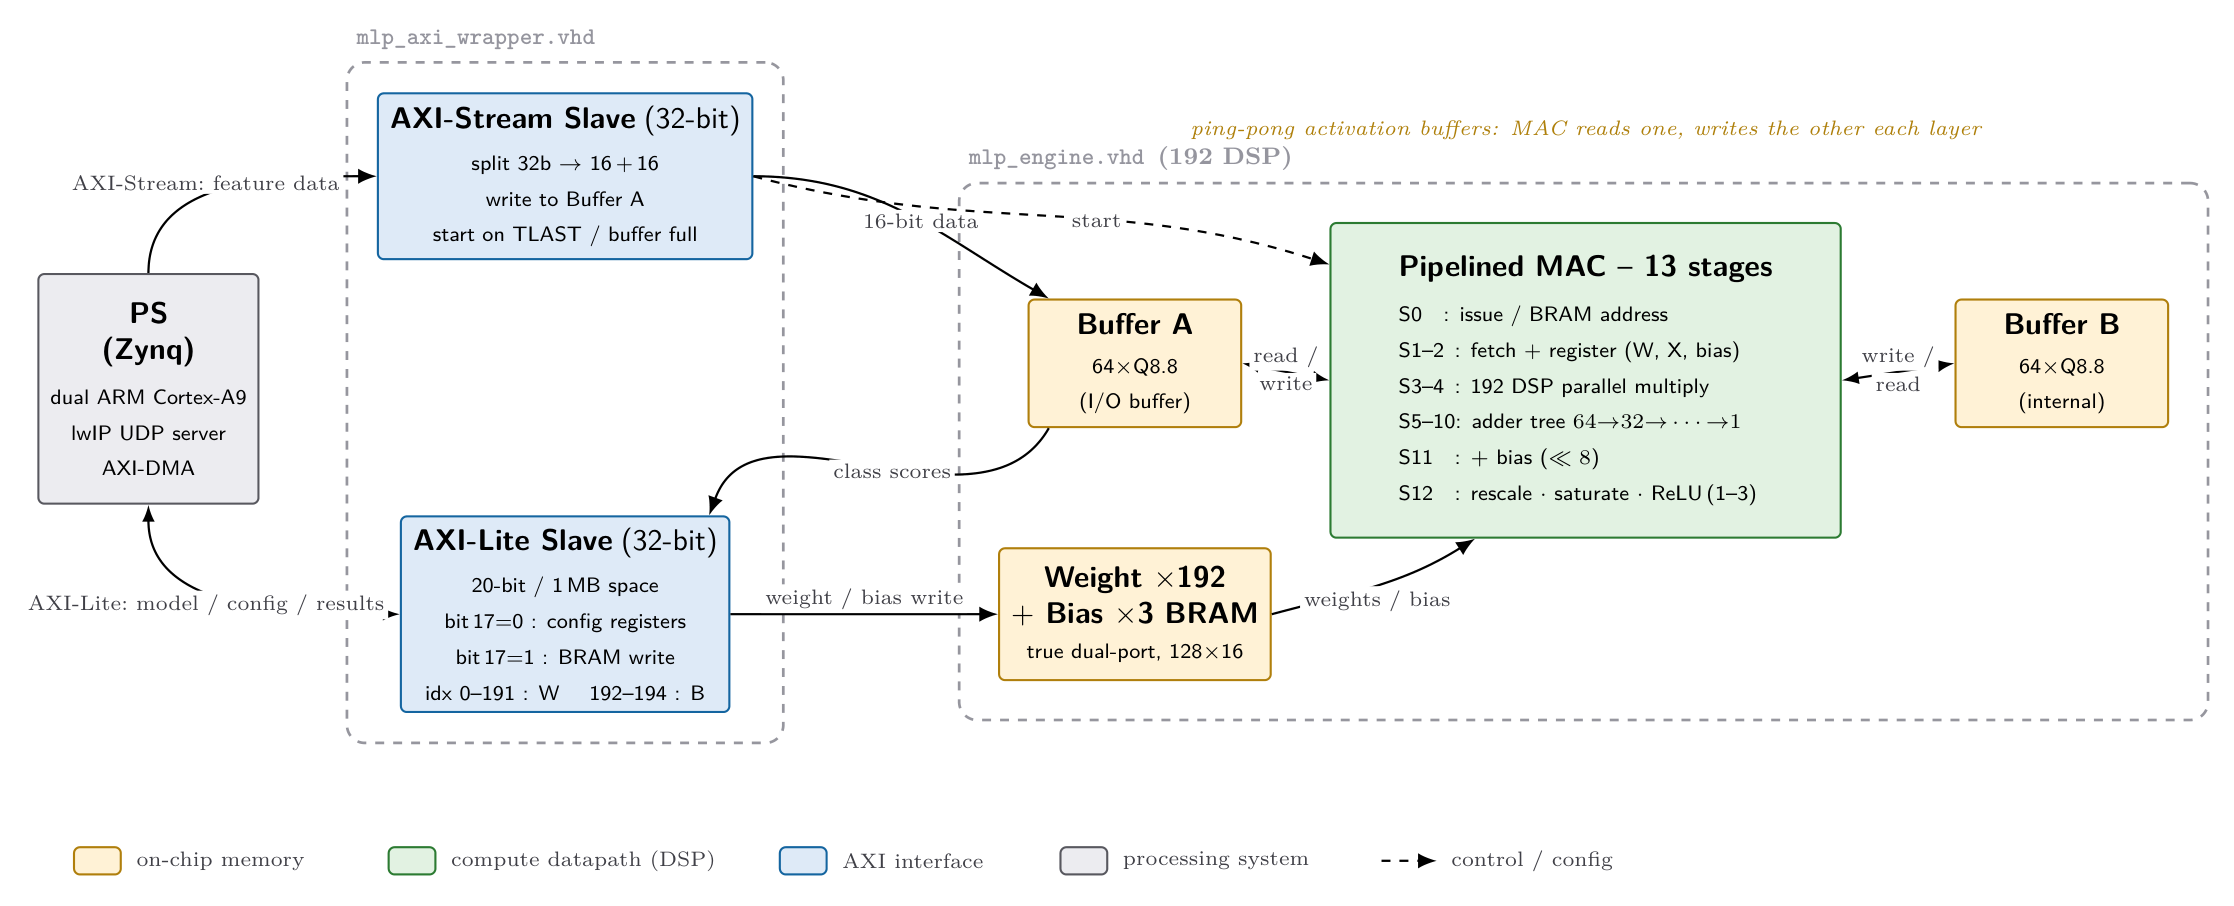
\includegraphics[width=0.92\textwidth]{figures/system_architecture.png}
\caption{System architecture of the proposed framework on the Zynq-7000 SoC.
Market data arrives over Ethernet at the PS, which forwards the prepared
feature vector to the custom \texttt{mlp\_axi\_wrapper} core through
AXI-DMA / AXI-Stream; the model parameters are loaded and the final decision
is read back over AXI-Lite. The entire inference is executed by the 13-stage
pipelined MAC engine in the PL.}
\label{fig:block_design}
\end{figure*}

\subsection{Ethernet-Enabled Data Path}
Feature packets are delivered over Ethernet to the PS, parsed, and forwarded to
the PL. Each 32-bit AXI-Stream word carries two 16-bit $Q8.8$ values, and the 40
features, zero-padded to the 64-wide datapath, are transferred as 32 stream
words on which the engine auto-starts. Table~\ref{tab:ethernet_measurement_plan}
lists the per-stage measurement points for the Ethernet-to-decision path; every
stage is instrumented and quantified over a 1{,}004{,}229-packet run in
Section~\ref{sec:eval} (Table~\ref{tab:latency_breakdown}).

\begin{table}[htbp]
\centering
\caption{Ethernet-enabled data path measurement plan}
\label{tab:ethernet_measurement_plan}
\begin{tabular}{p{3.2cm} p{4.2cm}}
\toprule
Metric & Description \\
\midrule
Packet receive latency & PS-side NIC-to-buffer time, $\approx$\SI{7.6}{\micro\second} \\
Packet parsing latency & Feature extraction in PS, $\approx$\SI{0.7}{\micro\second} \\
DMA transfer latency & AXI-DMA PS$\rightarrow$PL transfer, $\approx$\SI{3.7}{\micro\second} \\
MLP inference latency & PL core, \SI{768}{\nano\second} (Sec.~\ref{sec:eval}) \\
Packet-to-decision latency & Full end-to-end, $\approx$\SI{68.6}{\micro\second} \\
\bottomrule
\end{tabular}
\end{table}

\subsection{Customization Flow}
The framework is reusable across models and strategies. A user trains an MLP on
their own dataset and feature set; the trained parameters are quantized and the
on-chip weight/bias memories are regenerated, while the datapath, AXI
interfaces, and control logic are unchanged. Table~\ref{tab:customization_options}
summarizes the configurable components.

\begin{table}[htbp]
\centering
\caption{Customization options supported by the proposed framework}
\label{tab:customization_options}
\begin{tabular}{p{3.0cm} p{4.4cm}}
\toprule
Component & Customizable Parameters \\
\midrule
Input features & Feature vector contents and size (default 40) \\
MLP model & Retrainable weights/biases; hidden-layer sizes \\
Fixed-point format & Word/fraction split (default $Q8.8$) \\
Output decision & Class set, e.g.\ BUY / HOLD / SELL \\
Deployment flow & Automatic weight/bias memory regeneration \\
\bottomrule
\end{tabular}
\end{table}

%%%%%%%%%%%%%%%%%%%%%%%%%%%%%%%%%%%%%%%%%%%%%%%%%%%%%%%%%%%%%%%%%%%%%%%%%%%%%%%
\section{FPGA-Embedded Neural Inference Architecture}
%%%%%%%%%%%%%%%%%%%%%%%%%%%%%%%%%%%%%%%%%%%%%%%%%%%%%%%%%%%%%%%%%%%%%%%%%%%%%%%
The embedded network is an MLP with topology
$40\!\rightarrow\!64\!\rightarrow\!32\!\rightarrow\!16\!\rightarrow\!3$: a
40-dimensional input feature vector, three hidden layers with ReLU activation,
and a 3-class output (BUY/HOLD/SELL); the argmax over the three raw scores is
evaluated by the PS after read-back.
Inference is performed entirely in hardware; no layer is offloaded to the PS.

\subsection{Fixed-Point Quantization}
The floating-point model is converted to a $Q8.8$ fixed-point representation
(8 integer, 8 fractional bits), which lowers resource usage and enables
single-cycle DSP multiplications while preserving accuracy. Weights and biases
are stored in BRAM and addressed through the AXI-Lite configuration interface.
Table~\ref{tab:quantization_eval} reports the effect of quantization on the
reference model. The fidelity of the \emph{hardware} implementation of this
arithmetic is a separate question and is established independently in
Section~\ref{sec:verification}.

\begin{table}[htbp]
\centering
\caption{Effect of $Q8.8$ quantization on the reference model}
\label{tab:quantization_eval}
\begin{tabular}{p{3.1cm} p{4.3cm}}
\toprule
Metric & Value \\
\midrule
Float accuracy & 61.74\% \\
$Q8.8$ accuracy & 61.65\% \\
$Q8.8$ vs.\ float agreement & 99.93\% (macro F1 0.990) \\
Class change ratio (float vs.\ $Q8.8$) & 0.074\% \\
\bottomrule
\end{tabular}
\end{table}

\subsection{Parallel MAC-Based Inference Core}
The inference core (\texttt{mlp\_engine}) is built around 192 DSP slices used as
parallel multipliers; the accumulation is not performed inside the DSP blocks but
by a fabric adder tree, which is why the logic utilization is dominated by the
reduction network rather than by the multiplications, organized as a 13-stage
pipeline (Fig.~\ref{fig:microarch}): one address-issue stage (S0) followed by
twelve datapath stages. Stages 1 and 2 read weights/inputs from BRAM
and register them; stages 3 and 4 perform the 192 parallel multiplications;
stages 5 to 10 reduce the products through a balanced $64\!\rightarrow\!1$ adder
tree; stage 11 adds the bias; and stage 12 rescales the result and applies the
ReLU activation before write-back.
Two ping-pong buffers (Buffer~A / Buffer~B) hold the inter-layer activations so
that successive layers reuse the same MAC array.

\begin{figure*}[t]
\centering
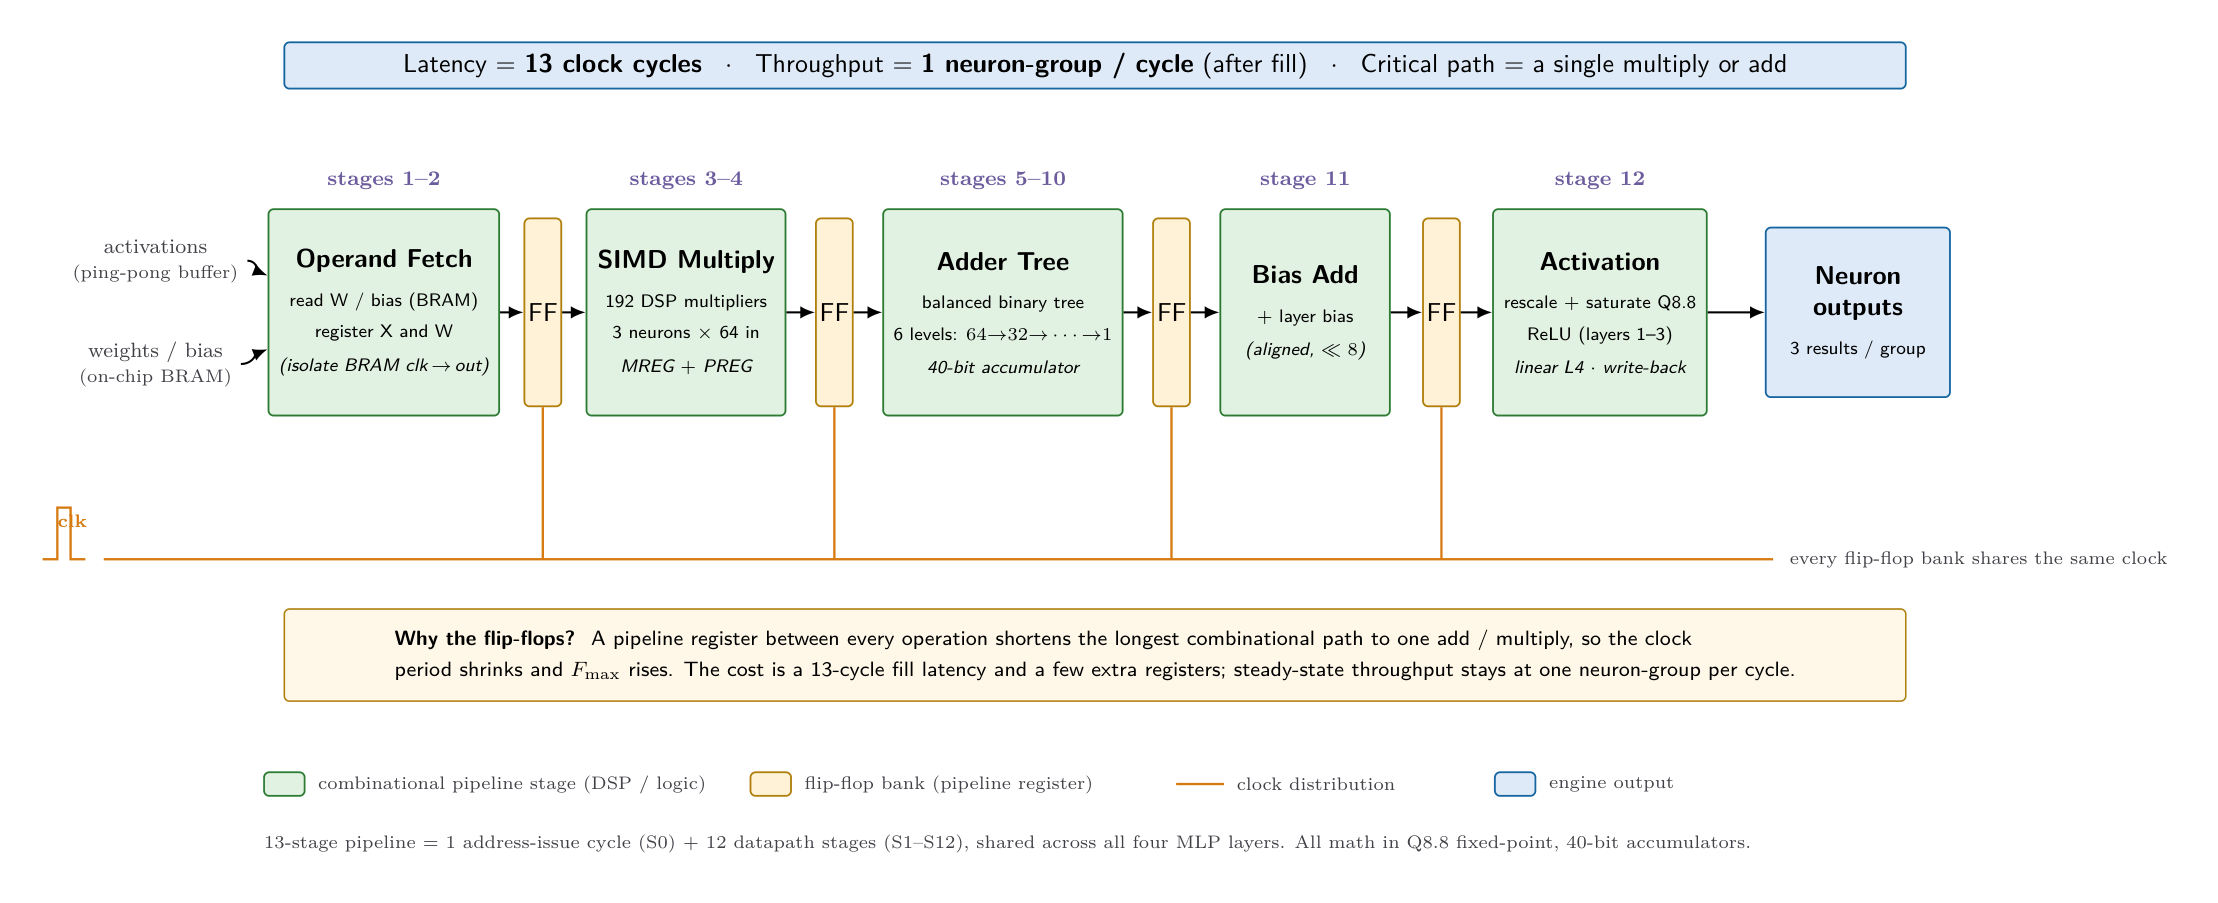
\includegraphics[width=0.92\textwidth]{figures/mlp_engine_pipeline.png}
\caption{Pipeline datapath of the hardware MLP core (\texttt{mlp\_engine}).
After the address-issue stage (S0), stages 1 and 2 fetch the weights, inputs, and
bias from BRAM; stages 3 and 4 perform the 192 parallel $Q8.8$ multiplications on
the DSP slices; stages 5 to 10 form the balanced $64\!\rightarrow\!1$ adder tree;
stage 11 adds the bias; and stage 12 rescales and applies the ReLU before the
result is written back to the ping-pong activation buffers. The
\texttt{mlp\_axi\_wrapper} splits each 32-bit AXI-Stream word into two 16-bit
$Q8.8$ values and triggers the engine; weights/biases reside in BRAM and are
loaded via AXI-Lite (address bit~17 selects configuration vs.\ memory).}
\label{fig:microarch}
\end{figure*}

%%%%%%%%%%%%%%%%%%%%%%%%%%%%%%%%%%%%%%%%%%%%%%%%%%%%%%%%%%%%%%%%%%%%%%%%%%%%%%%
\section{Implementation on Zynq-7000 SoC}
%%%%%%%%%%%%%%%%%%%%%%%%%%%%%%%%%%%%%%%%%%%%%%%%%%%%%%%%%%%%%%%%%%%%%%%%%%%%%%%

\subsection{Hardware/Software Partitioning}
Table~\ref{tab:hw_sw_partitioning} lists where each function is implemented.
The PL implements the entire inference datapath and the measurement signals; the
PS is responsible for the network interface, for handing the received feature
vector to the DMA engine, and for high-level control.

Two aspects of this partition should be stated plainly, because they bound what
the reported latency covers. First, feature construction and the conversion to
$Q8.8$ are performed \emph{upstream of the board}: the packet arriving at the PS
already contains a quantized, zero-padded vector, and the PS copies it into a
DMA-aligned buffer without transforming it. Moving feature construction onto the
PS would add work to the measured path and is not claimed here. Second, the
argmax over the three output scores is evaluated in PS software after the scores
have been read back over AXI-Lite; it is a three-way comparison and is included
in the read-out stage of the latency breakdown
(Table~\ref{tab:latency_breakdown}) rather than in the core latency. Moving it
into the PL would remove two of the three AXI-Lite reads and is a
straightforward extension.

\begin{table}[t]
\centering
\caption{Hardware/software partitioning of the proposed system}
\label{tab:hw_sw_partitioning}
\begin{tabular}{p{2.8cm} p{4.6cm}}
\toprule
Component & Implementation Location \\
\midrule
Ethernet packet reception & PS (software) \\
Feature vector hand-off & PS (software, \texttt{memcpy}) \\
Feature vector transfer & AXI-DMA (PS$\rightarrow$PL) \\
MLP inference & PL (hardware) \\
Argmax decision & PS (software, after read-back) \\
Status/result registers & AXI-Lite (PS$\leftrightarrow$PL) \\
Debug signals & PL output pins \\
\bottomrule
\end{tabular}
\end{table}

\subsection{AXI-Stream and AXI-DMA Interface}
The PS prepares the feature vector and transfers it to the PL with AXI-DMA; the
\texttt{mlp\_axi\_wrapper} consumes it as an AXI-Stream slave, splitting each
32-bit word into two $Q8.8$ operands and starting the engine once a full vector
is received. Control and status (start, busy, done, result) use AXI-Lite. This
keeps the inference pipeline continuously fed without per-operand PS
intervention.

\subsection{Debug and Measurement Infrastructure}
To measure hardware timing directly, the core exports the dedicated debug
signals of Table~\ref{tab:debug_signals}. \texttt{dbg\_data\_in\_pulse} marks
the arrival of a complete feature vector, \texttt{dbg\_layer1\_done} to \texttt{dbg\_layer4\_done} pulse as
each layer finishes, and \texttt{dbg\_mlp\_busy} brackets the whole inference.
These pins are probed with an oscilloscope, so the per-layer latency is observed
on real silicon rather than estimated (Section~\ref{sec:eval}).

\begin{table}[htbp]
\centering
\caption{Debug signals exported for hardware latency measurement. All signal
names carry the prefix \texttt{dbg\_}, omitted here for space.}
\label{tab:debug_signals}
\small
\begin{tabular}{@{}L{2.3cm}L{5.0cm}@{}}
\toprule
Signal & Purpose \\
\midrule
\texttt{data\_in\_pulse} & Full feature vector received \\
\texttt{layer1\_done}    & Layer 1 ($40\!\rightarrow\!64$) complete \\
\texttt{layer2\_done}    & Layer 2 ($64\!\rightarrow\!32$) complete \\
\texttt{layer3\_done}    & Layer 3 ($32\!\rightarrow\!16$) complete \\
\texttt{layer4\_done}    & Layer 4 ($16\!\rightarrow\!3$) complete \\
\texttt{mlp\_busy}       & Inference in progress; decision valid on the falling edge \\
\bottomrule
\end{tabular}
\end{table}

%%%%%%%%%%%%%%%%%%%%%%%%%%%%%%%%%%%%%%%%%%%%%%%%%%%%%%%%%%%%%%%%%%%%%%%%%%%%%%%
\section{Experimental Evaluation}
\label{sec:eval}
%%%%%%%%%%%%%%%%%%%%%%%%%%%%%%%%%%%%%%%%%%%%%%%%%%%%%%%%%%%%%%%%%%%%%%%%%%%%%%%

\subsection{Experimental Setup}
The framework is implemented on a Xilinx Zynq-7000 SoC. A host control
application (Fig.~\ref{fig:gui}) connects to the C++ host engine, uploads the
quantized model, and streams either real CSV market data or randomized test
packets while reporting the last prediction, last latency, and processed-packet
count. Table~\ref{tab:experimental_setup} summarizes the setup.

\begin{figure}[t]
\centering
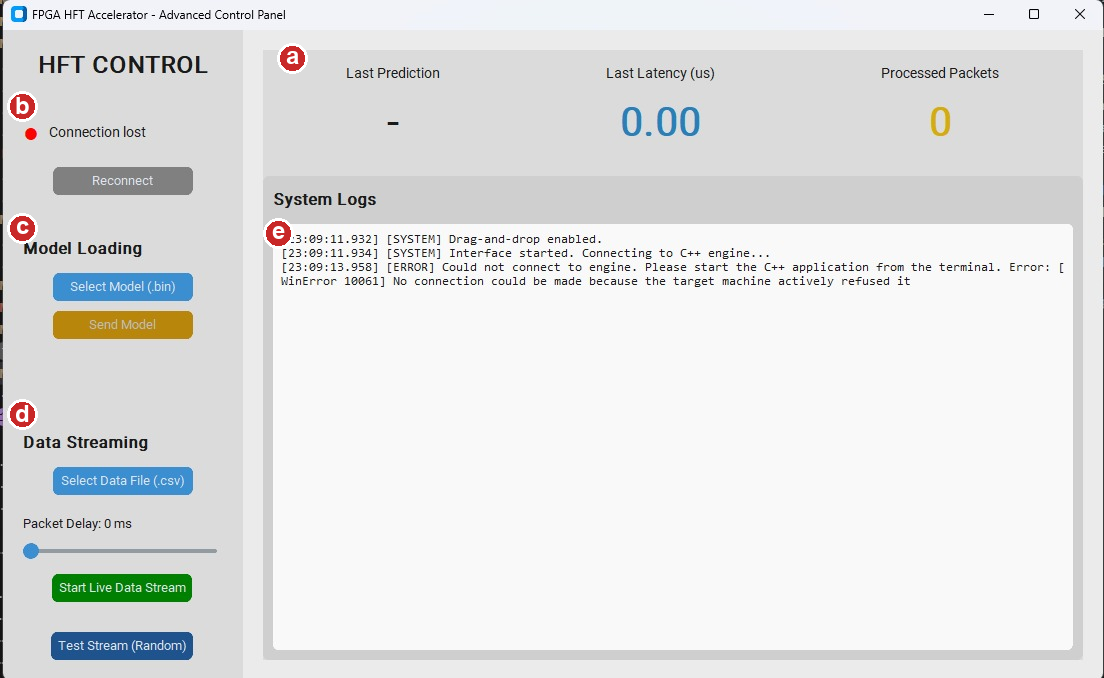
\includegraphics[width=\linewidth]{figures/host_gui_annotated.png}
\caption{Host control application used to configure, drive, and validate the
FPGA inference system. (a) Real-time dashboard showing the last predicted
decision, the last measured round-trip latency in microseconds, and the number
of processed packets. (b) Engine connection status and reconnect control,
indicating whether the host is connected to the inference engine. (c)
Model-loading panel, used to select a trained model (\texttt{.bin}) and upload
it to the board over the network. (d) Data-streaming panel, used to select a
recorded CSV dataset, set the inter-packet delay, and start either a live
stream or a randomized test stream. (e) System-log console, which reports
connection events, errors, and run-time messages during operation.}
\label{fig:gui}
\end{figure}

\begin{table}[t]
\centering
\caption{Experimental setup}
\label{tab:experimental_setup}
\begin{tabular}{p{3.1cm} p{4.3cm}}
\toprule
Item & Description \\
\midrule
FPGA device & Xilinx XC7Z020-1CLG484 (ZedBoard) \\
Design language & VHDL (PL); C++/Python (PS/host) \\
Tool version & Xilinx Vivado / Vitis 2025.2 \\
PS software & Bare-metal, lwIP raw API (no OS on the board) \\
Data path & Ethernet $\to$ PS $\to$ AXI-DMA $\to$ AXI-Stream $\to$ PL \\
Inference core & MLP $40$-$64$-$32$-$16$-$3$, $Q8.8$, 192 DSP MACs \\
Test size & 120{,}883 inference requests (Linux end-to-end) \\
Clock frequency & \SI{125}{\mega\hertz} (PL) \\
\bottomrule
\end{tabular}
\end{table}

%%%%%%%%%%%%%%%%%%%%%%%%%%%%%%%%%%%%%%%%%%%%%%%%%%%%%%%%%%%%%%%%%%%%%%%%%%%%%%%
\subsection{Functional Verification of the Inference Core}
\label{sec:verification}
%%%%%%%%%%%%%%%%%%%%%%%%%%%%%%%%%%%%%%%%%%%%%%%%%%%%%%%%%%%%%%%%%%%%%%%%%%%%%%%
Reporting latency and resource figures for an accelerator is only meaningful if
the accelerator is first shown to compute the intended function. We therefore
verify the core at three levels before reporting any performance result.

\paragraph{Golden reference model.}
A bit-accurate software model of the datapath was written independently of the
RTL. It reproduces every arithmetic detail of the deployed pipeline: the host
$Q8.8$ conversion with saturation, the truncating weight conversion performed by
the on-board loader, the 40-bit accumulation, the arithmetic right shift, the
16-bit saturation, the ReLU on all but the output layer, and the argmax rule
used by the decision logic. A second, cycle-accurate model of
\texttt{mlp\_engine} was also written; it reproduces the issue FSM, the 13-stage
token pipeline, the one-cycle BRAM read latency and the ping-pong write-back,
and it is used to reason about pipeline alignment independently of the
simulator.

\paragraph{Directed RTL simulation.}
Three directed tests exercise mutually independent mechanisms of the engine: a
pass-through chain that isolates the multiply, reduce and rescale datapath, a
bias-only chain that isolates the bias pipeline, and a multi-neuron test that
isolates the write-back indexing. Each test writes its parameters through the
same AXI-Lite address map used by the on-board loader, streams a stimulus vector
over AXI-Stream, and compares the three read-back outputs against values
computed by hand. Input positions that are not overwritten by the network are
pre-loaded with distinctive values, so that a missing write-back cannot be
mistaken for a correct result.

This step exposed three pipeline-alignment defects in the original design that
were invisible to synthesis and to end-to-end testing
(Table~\ref{tab:rtl_defects}). All three are one-line index corrections; none
changes the pipeline depth, the resource usage or the timing closure of the
design. After correction, the cycle-accurate model matched the golden reference
on 240 randomly generated cases (60 random parameter sets $\times$ 4 random
input vectors), whereas the original alignment matched on none.

\begin{table}[htbp]
\centering
\caption{Pipeline-alignment defects found by directed simulation}
\label{tab:rtl_defects}
\small
\begin{tabular}{@{}p{2.0cm}p{1.0cm}p{4.4cm}@{}}
\toprule
Signal & Stage & Consequence \\
\midrule
Bias pipeline & $11\!\rightarrow\!9$ & Each neuron received the bias of a neuron six positions earlier \\
Write-back token & $12\!\rightarrow\!11$ & Results were written to the wrong activation indices \\
Input multiplexer & $2\!\rightarrow\!1$ & Each layer read from the wrong ping-pong buffer \\
\bottomrule
\end{tabular}
\end{table}

\paragraph{On-hardware bit-exact verification.}
The corrected design was verified on the board against the golden model over a
stimulus set constructed to exercise the saturation, ReLU, sign-transition and
zero-padding paths, rather than over recorded market data whose dynamic range
does not span the $Q8.8$ interval. The firmware was extended to return the three
raw 16-bit output values alongside the decision, so that the comparison is
made on the arithmetic itself and not only on the argmax.

Table~\ref{tab:verification} reports the result. Across four networks the
hardware reproduced the golden model on 400{,}000 inferences and on all
1{,}200{,}000 raw output values, without a single discrepancy. We note that
agreement on the decision alone would be a weak check when the output
distribution is concentrated on one class; the per-output comparison is reported
for this reason.

\begin{table}[htbp]
\centering
\caption{On-hardware bit-exact verification against the golden model. All four
networks were loaded at run time into the \emph{same} bitstream. The last column
compares the three raw 16-bit outputs of every inference, i.e.\ 1{,}200{,}000
individual comparisons in total, none of which differed.}
\label{tab:verification}
\small
\begin{tabular}{@{}lrrr@{}}
\toprule
Network & Inferences & Decision & Outputs \\
\midrule
$40$-$64$-$32$-$16$-$3$ & 100{,}000 & 100.0000\% & 100.0000\% \\
$40$-$64$-$64$-$32$-$3$ & 100{,}000 & 100.0000\% & 100.0000\% \\
$40$-$32$-$16$-$8$-$3$  & 100{,}000 & 100.0000\% & 100.0000\% \\
$40$-$10$-$16$-$8$-$3$  & 100{,}000 & 100.0000\% & 100.0000\% \\
\midrule
Total                   & 400{,}000 & 100.0000\% & 100.0000\% \\
\bottomrule
\end{tabular}
\end{table}

\subsection{Model Accuracy and Classification Performance}
Table~\ref{tab:model_performance} reports, for the five trained models, the
accuracy obtained in floating point under PyTorch alongside the accuracy of the
same model executed on the FPGA in $Q8.8$. The two agree to within 0.22
percentage points, and to within 0.1 percentage points for the reference model.

The interpretation of this agreement should be stated carefully. It shows that
reducing the arithmetic to $Q8.8$ does not materially change the decisions the
network makes; it is a statement about the numerical format, not about the
predictive quality of the models themselves, and not about the correctness of
the hardware. The latter is established independently and exactly in
Section~\ref{sec:verification}.

\begin{table}[htbp]
\centering
\caption{PyTorch (float) vs.\ FPGA ($Q8.8$) accuracy for the five trained
models; the last column is the absolute accuracy difference in percentage
points.}
\label{tab:model_performance}
\begin{tabular}{lccc}
\toprule
Model & PyTorch Acc & FPGA Acc & Difference \\
\midrule
Model A & 61.74\% & 61.65\% & 0.0926 \\
Model B & 60.58\% & 60.59\% & 0.0164 \\
Model C & 60.62\% & 60.54\% & 0.0791 \\
Model D & 57.10\% & 56.88\% & 0.2174 \\
Model E & 56.86\% & 57.01\% & 0.1470 \\
\bottomrule
\end{tabular}
\end{table}

\subsection{System-Level Packet-to-Decision Latency}
Table~\ref{tab:latency_metrics} reports the measured end-to-end
packet-to-decision latency of the full FPGA system on the Linux host over
120{,}883 inference requests. Each request is a UDP round trip from the host to
the board and back, so it includes the network, the PS software, the AXI-DMA
transfer, and the PL core. The median is \SI{66.3}{\micro\second}; the pure
hardware core (Section~\ref{sec:eval}, \SI{768}{\nano\second}) is therefore
about \SI{1}{\percent} of the end-to-end time, confirming that the remaining
cost is dominated by the operating system, the network, and the PS software
rather than by the inference itself.

\begin{table}[htbp]
\centering
\caption{Measured end-to-end packet-to-decision latency of the FPGA system
(Linux host, 120{,}883 requests)}
\label{tab:latency_metrics}
\begin{tabular}{lc}
\toprule
Metric & Latency \\
\midrule
Minimum & \SI{50.0}{\micro\second} \\
Median & \SI{66.3}{\micro\second} \\
Mean & \SI{65.6}{\micro\second} \\
99th Percentile & \SI{79.6}{\micro\second} \\
99.9th Percentile & \SI{109.7}{\micro\second} \\
Maximum & \SI{3275.9}{\micro\second} \\
\bottomrule
\end{tabular}
\end{table}

\subsection{Sensitivity of the End-to-End Path to the Host Network Stack}
\label{sec:osbaseline}
The experiment in this subsection isolates how much of the end-to-end latency is
attributable to the host rather than to the board. It is not a software baseline
for the inference itself: the network is executed in the fabric in both runs, and
what changes is only the operating system driving the socket. A comparison
against a software implementation of the same network is given separately in
Section~\ref{sec:baseline}.

The same UDP round-trip run was repeated on a Linux and a Windows host, with the
board, the bitstream and the model held fixed.
Figure~\ref{fig:lat_hist} shows the two latency distributions.
The Linux host completes a median request in \SI{66.3}{\micro\second} (p99
\SI{79.6}{\micro\second}), whereas the Windows host needs
\SI{476.3}{\micro\second} (p99 \SI{608.7}{\micro\second}) and exhibits a much
heavier tail (p99.9 \SI{1649}{\micro\second}) and occasional timeouts. This
roughly $7\times$ difference in median latency, obtained with the same board,
the same bitstream and the same model, bounds how much of the end-to-end figure
can be attributed to the host: at least a factor of seven of the median is
determined by software outside the board. The hardware core is unaffected, since its
latency is fixed by the pipeline depth and was measured as constant on the debug
pins. The variability seen here, and the heavy tail in particular,
originates entirely on the host side of the link. This is also the reason the
end-to-end figures in Table~\ref{tab:latency_metrics} should not be read as a
property of the accelerator.

\begin{figure}[htbp]
\centering
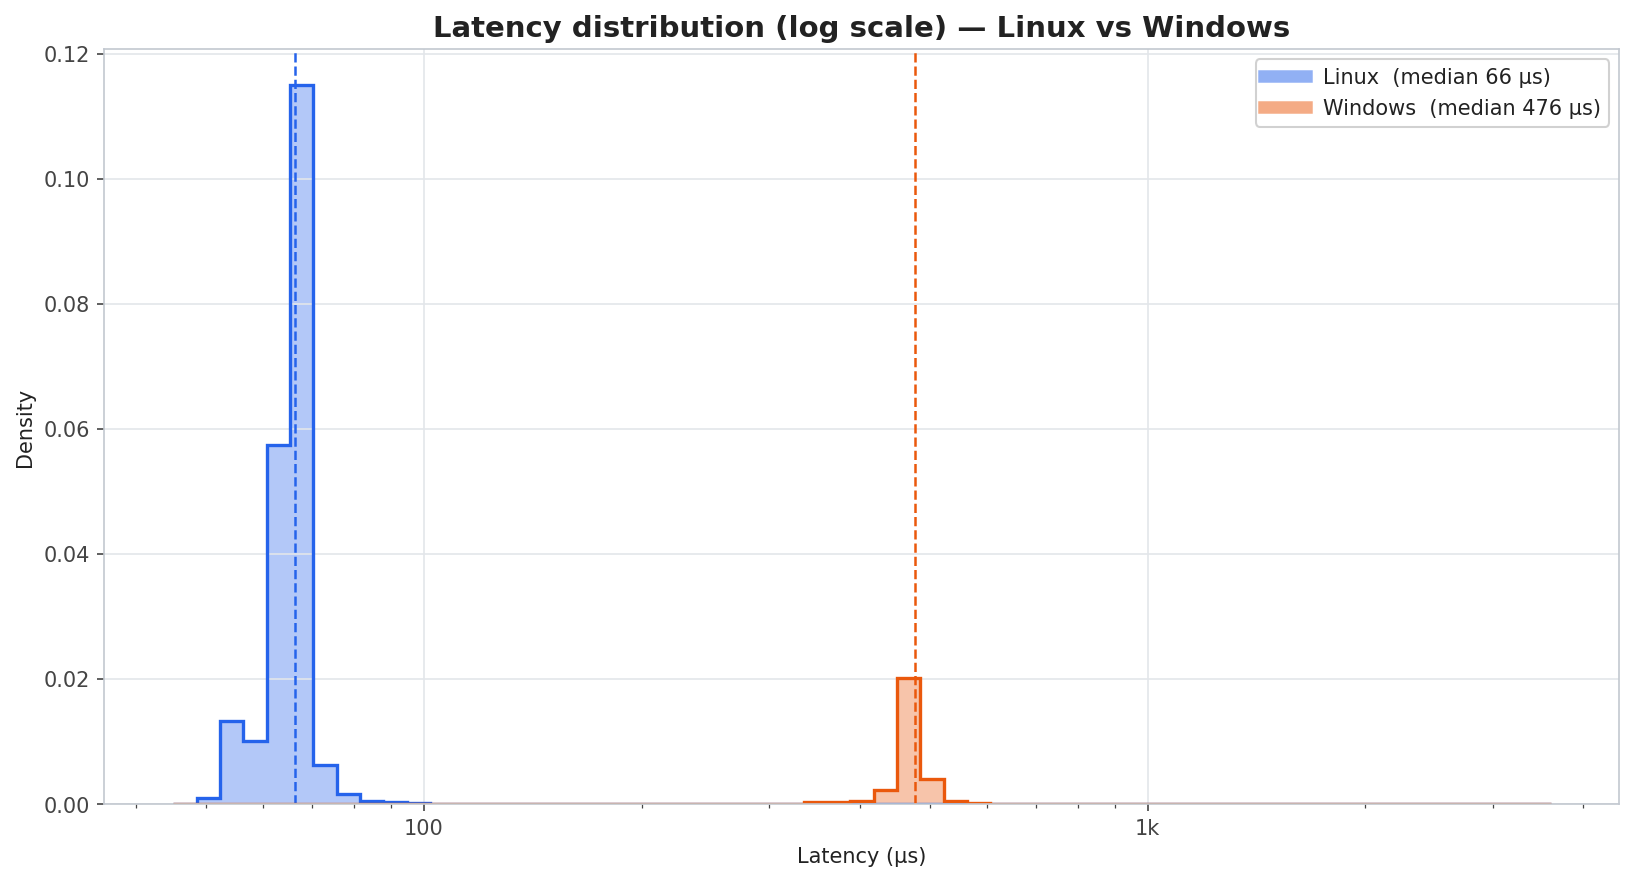
\includegraphics[width=\linewidth]{figures/lat_hist.png}
\caption{End-to-end latency distribution (log scale) on the Linux vs.\ Windows
host driving the same FPGA board. The OS-dependent gap and the heavier Windows
tail are evident.}
\label{fig:lat_hist}
\end{figure}

\subsection{Latency Breakdown}
Because each layer exposes a done pulse, the inference can be decomposed on real
hardware. Probing the debug pins with an oscilloscope yields the per-layer
inter-pulse times of Fig.~\ref{fig:scope_layer} and the total
input-to-final-done interval of Fig.~\ref{fig:scope_total}.
Table~\ref{tab:cycle_breakdown} converts these to clock cycles at
\SI{125}{\mega\hertz}. The measured per-layer times are 280, 200, 160,
and \SI{118}{\nano\second} for layers 1 to 4, and the measured end-to-end core
interval is \SI{768}{\nano\second}.

These values are not merely observed; they follow from the architecture. The
issue FSM emits one token per cycle while a layer is being issued, and each
token carries three neurons, so a layer of $n_\ell$ outputs occupies
$\lceil n_\ell/3 \rceil$ issue cycles. The FSM then waits for the pipeline to
empty before advancing, which costs the full pipeline depth. The per-layer
occupancy is therefore
%
\begin{equation}
c_\ell \;=\; \left\lceil \frac{n_\ell}{3} \right\rceil + D + 1,
\qquad D = 13,
\label{eq:cycles}
\end{equation}
%
where $D$ is the depth of the token pipeline. Table~\ref{tab:cycle_breakdown}
compares this prediction with the oscilloscope measurement. The predicted total,
$\sum_\ell c_\ell = 96$ cycles or \SI{768}{\nano\second}, agrees exactly with
the measured input-to-done interval. Two of the four individual intervals read
slightly below the prediction, layer~1 at \SI{280}{\nano\second} against a
predicted \SI{288}{\nano\second} and layer~4 at \SI{118}{\nano\second} against
\SI{120}{\nano\second}, so the four inter-pulse intervals sum to
\SI{758}{\nano\second} where the interval measured directly between the first
and last pulse is \SI{768}{\nano\second}. Both deviations are in the same
direction and neither exceeds one clock period. The per-layer figures come from
four separate captures in which one clock period occupies a small fraction of a
division, and a spread of \SI{10}{\nano\second} accumulated over four such
readings is consistent with that reading uncertainty. We therefore treat the
total, which is corroborated independently by the cycle counter of
Section~\ref{sec:determinism}, as the authoritative figure, and the per-layer
captures as confirming the model to within one cycle. Latching a counter at
each \texttt{layer\_done} would remove the ambiguity entirely and is the
appropriate instrument for per-layer timing at this resolution.

We note that the drain term in \eqref{eq:cycles} is not negligible: of the 96
cycles, 56 are spent draining the pipeline between layers rather than issuing
work, so only \SI{42}{\percent} of the core latency performs useful issue. This is a direct consequence of the ping-pong buffering, since a layer
cannot begin reading a buffer until the preceding layer has finished writing it.
For the narrow output layers the effect is pronounced: layer~4 issues a
single token and then drains for 13 cycles. Overlapping the drain of one layer
with the issue of the next would require double-buffering the activations at
sub-layer granularity and is left as future work; at the present operating point
the core latency is in any case a small fraction of the end-to-end path.

\paragraph{Arithmetic efficiency.}
The consequences for throughput are worth stating explicitly, since related work
is frequently compared on this basis. With 192 multipliers at
\SI{125}{\mega\hertz} the peak arithmetic rate is \SI{48}{GOP/s}. A single
inference of the reference network performs $40\!\times\!64 + 64\!\times\!32 +
32\!\times\!16 + 16\!\times\!3 = 5168$ useful multiply-accumulate operations,
but the zero-padded SIMD array issues 7680 multiplications, so
\SI{67}{\percent} of the issued arithmetic is useful. Combined with the drain
overhead, the achieved rate is $2 \times 5168 / \SI{768}{\nano\second} \approx
\SI{13.5}{GOP/s}$, or \SI{28}{\percent} of peak. The core sustains
\SI{1.30}{M} inferences per second; at system level the AXI-Stream wrapper does
not overlap the reception of one feature vector with the computation of the
previous one, which reduces the sustained rate to approximately
\SI{0.77}{M} inferences per second. Both figures are far in excess of what the
host-side path can supply (Section~\ref{sec:eval}), which is why the design is
latency-optimized rather than throughput-optimized.

The full end-to-end path was then instrumented with PS-side timestamps over
1{,}004{,}229 packets (Table~\ref{tab:latency_breakdown}). The result isolates
where the time is spent: of the \SI{68.6}{\micro\second} mean host-to-decision
latency, only \SI{14.4}{\micro\second} is spent on the board (PS + PL), and the
remaining \SI{54}{\micro\second} is host-side NIC, operating-system, and wire
time. On the board, the Ethernet reception (EMAC + lwIP) dominates and is
bimodal (p50 \SI{2.6}{\micro\second} vs p99 \SI{14.2}{\micro\second}), reflecting
the phase of the polling loop relative to packet arrival, whereas the DMA,
PL compute, and readout stages are tightly bounded (sub-microsecond to a few
microseconds, with p99 within a few percent of the median). This confirms the
central claim: the deterministic hardware core is a negligible and jitter-free
fraction of the end-to-end latency, and the remaining cost is host- and
network-side software, which a hardware Ethernet MAC in the PL would remove.

\begin{figure}[htbp]
\centering
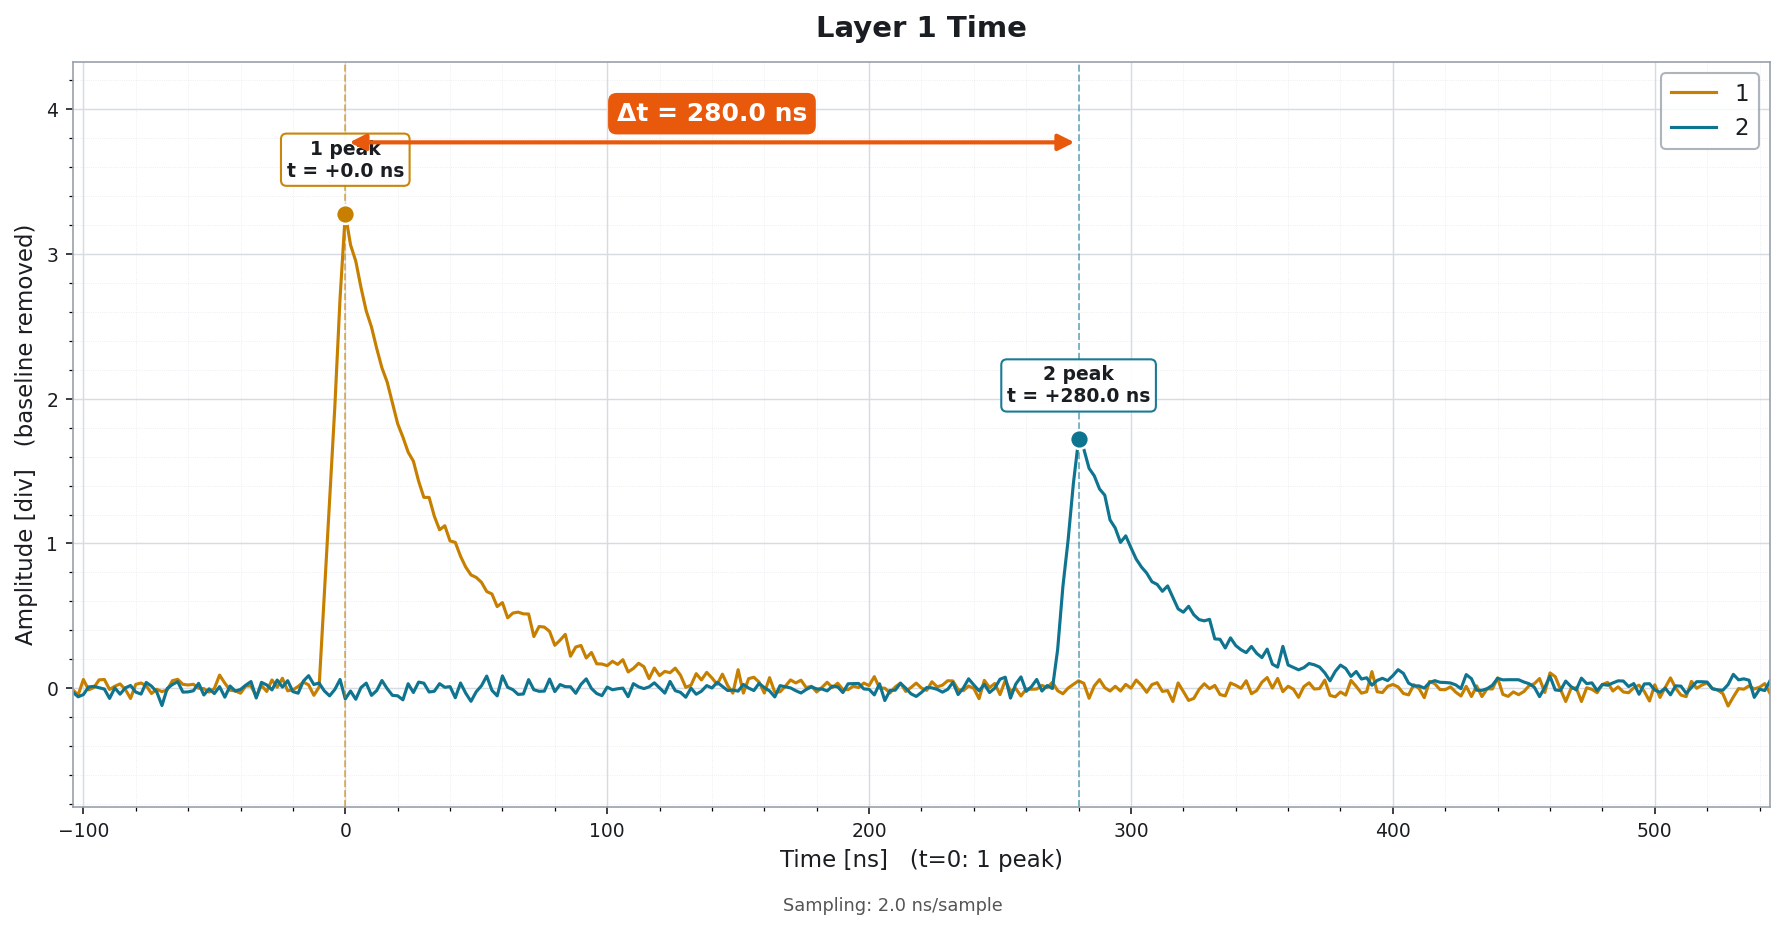
\includegraphics[width=0.49\linewidth]{figures/scope_layer1.png}\hfill
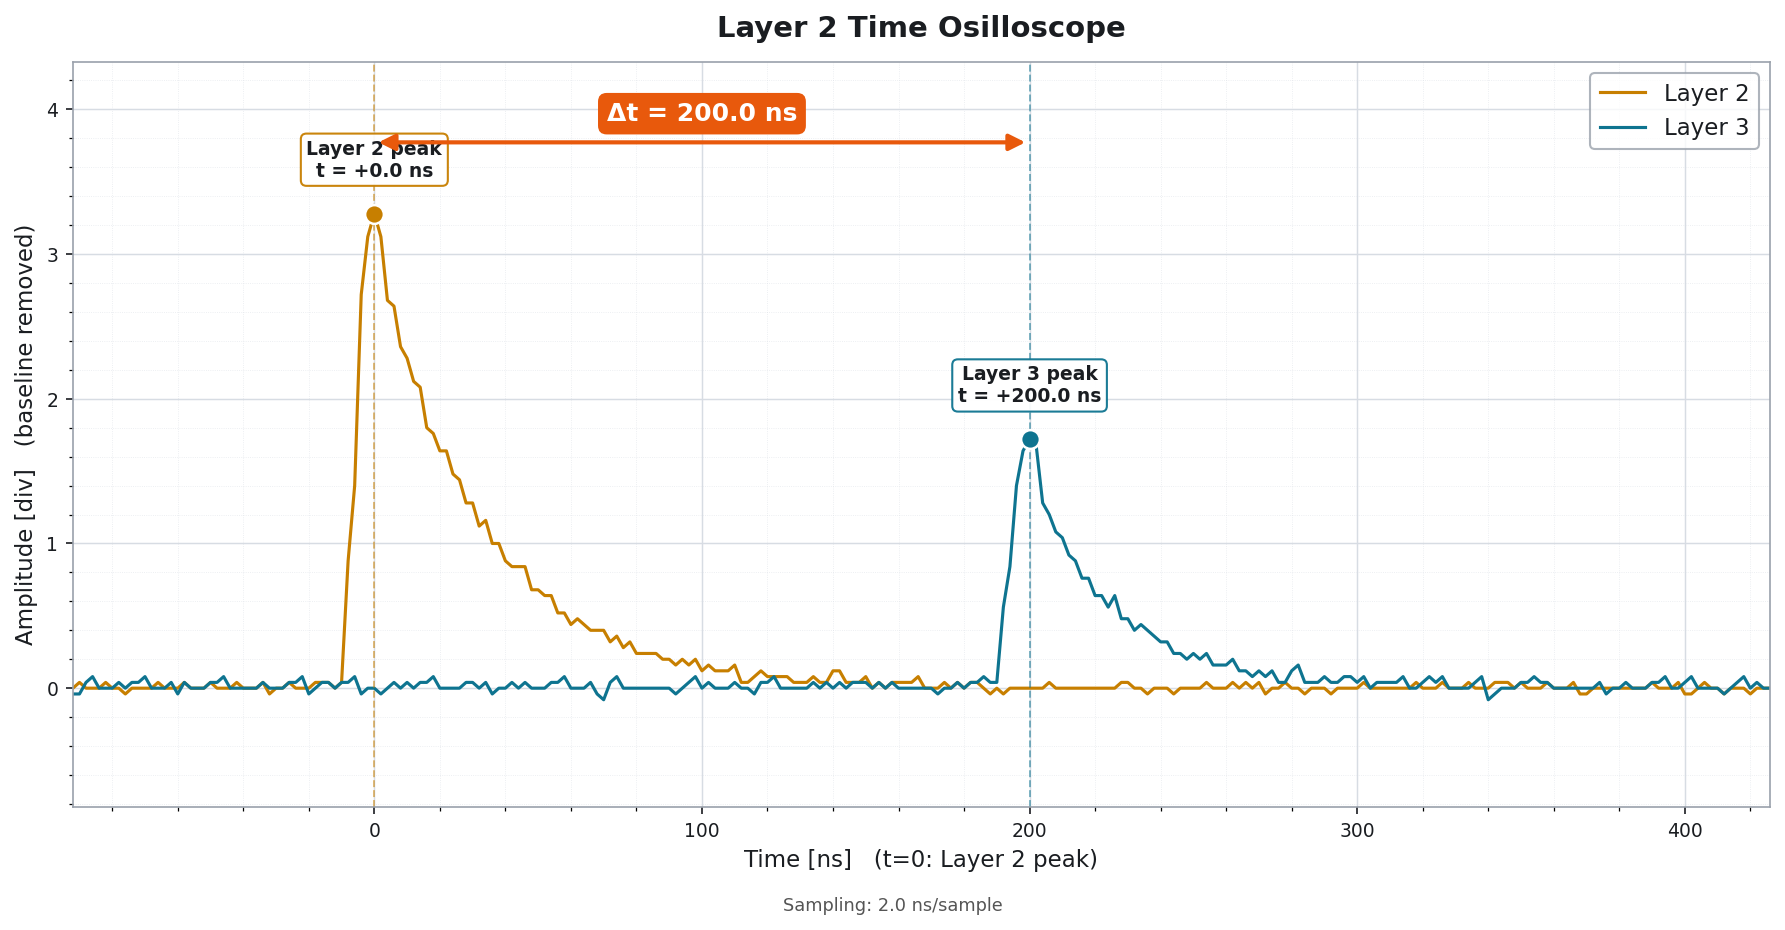
\includegraphics[width=0.49\linewidth]{figures/scope_layer2.png}\\[3pt]
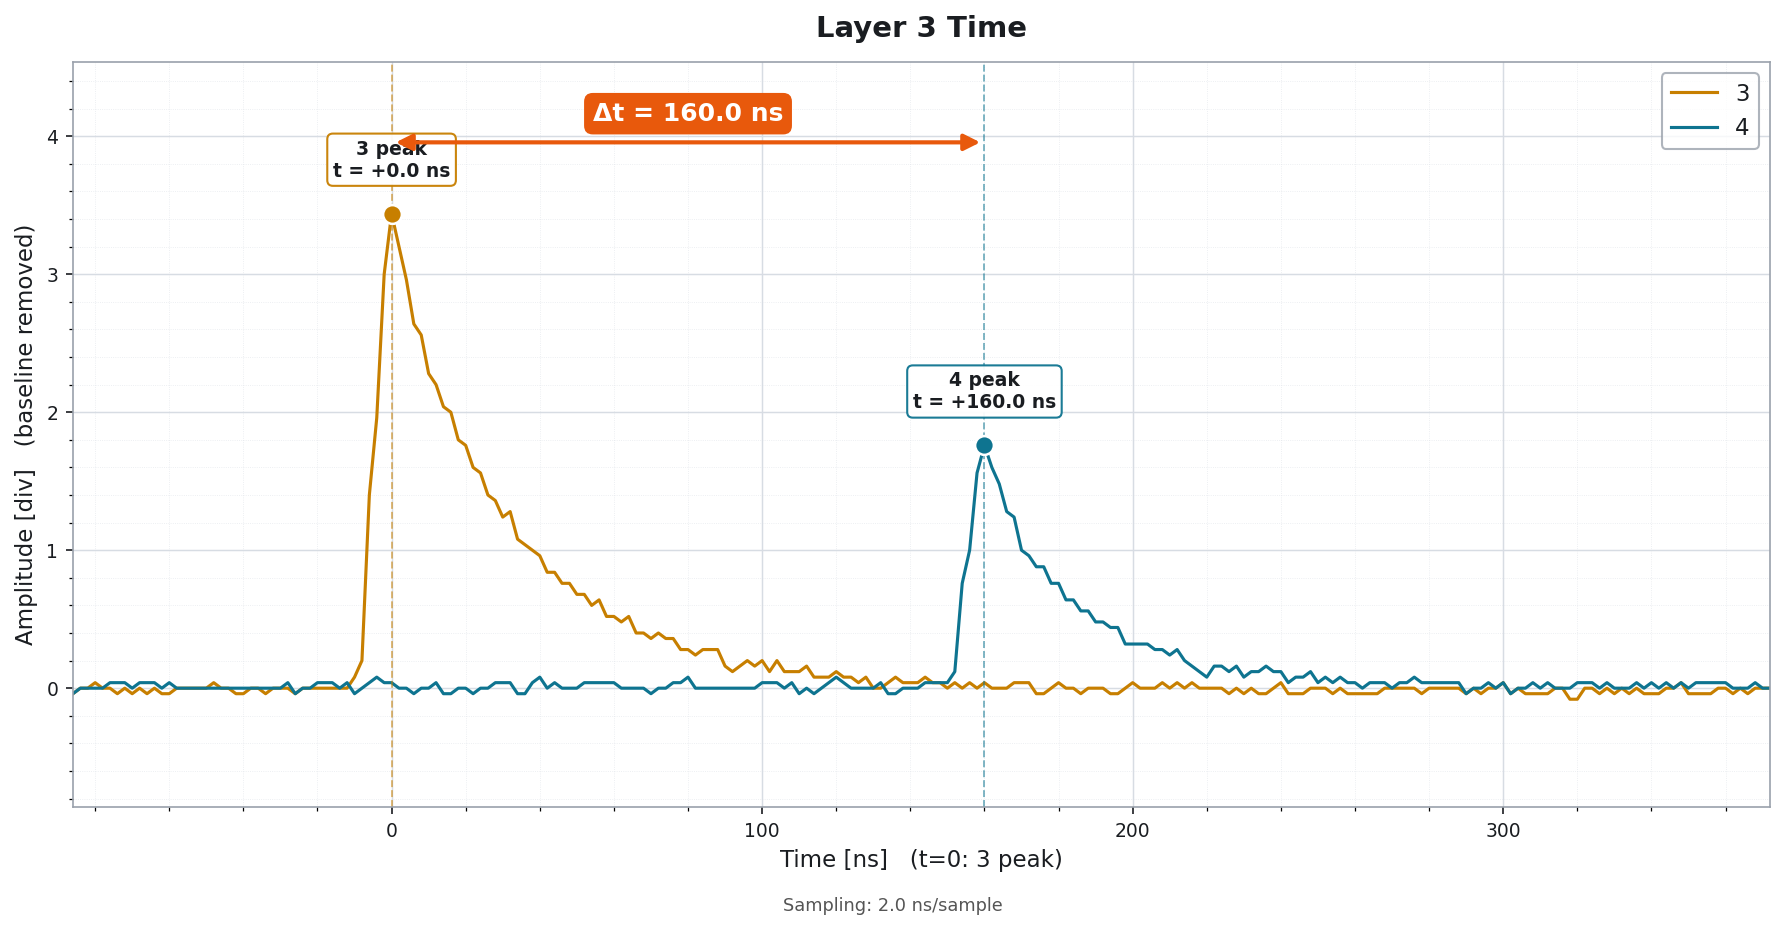
\includegraphics[width=0.49\linewidth]{figures/scope_layer3.png}\hfill
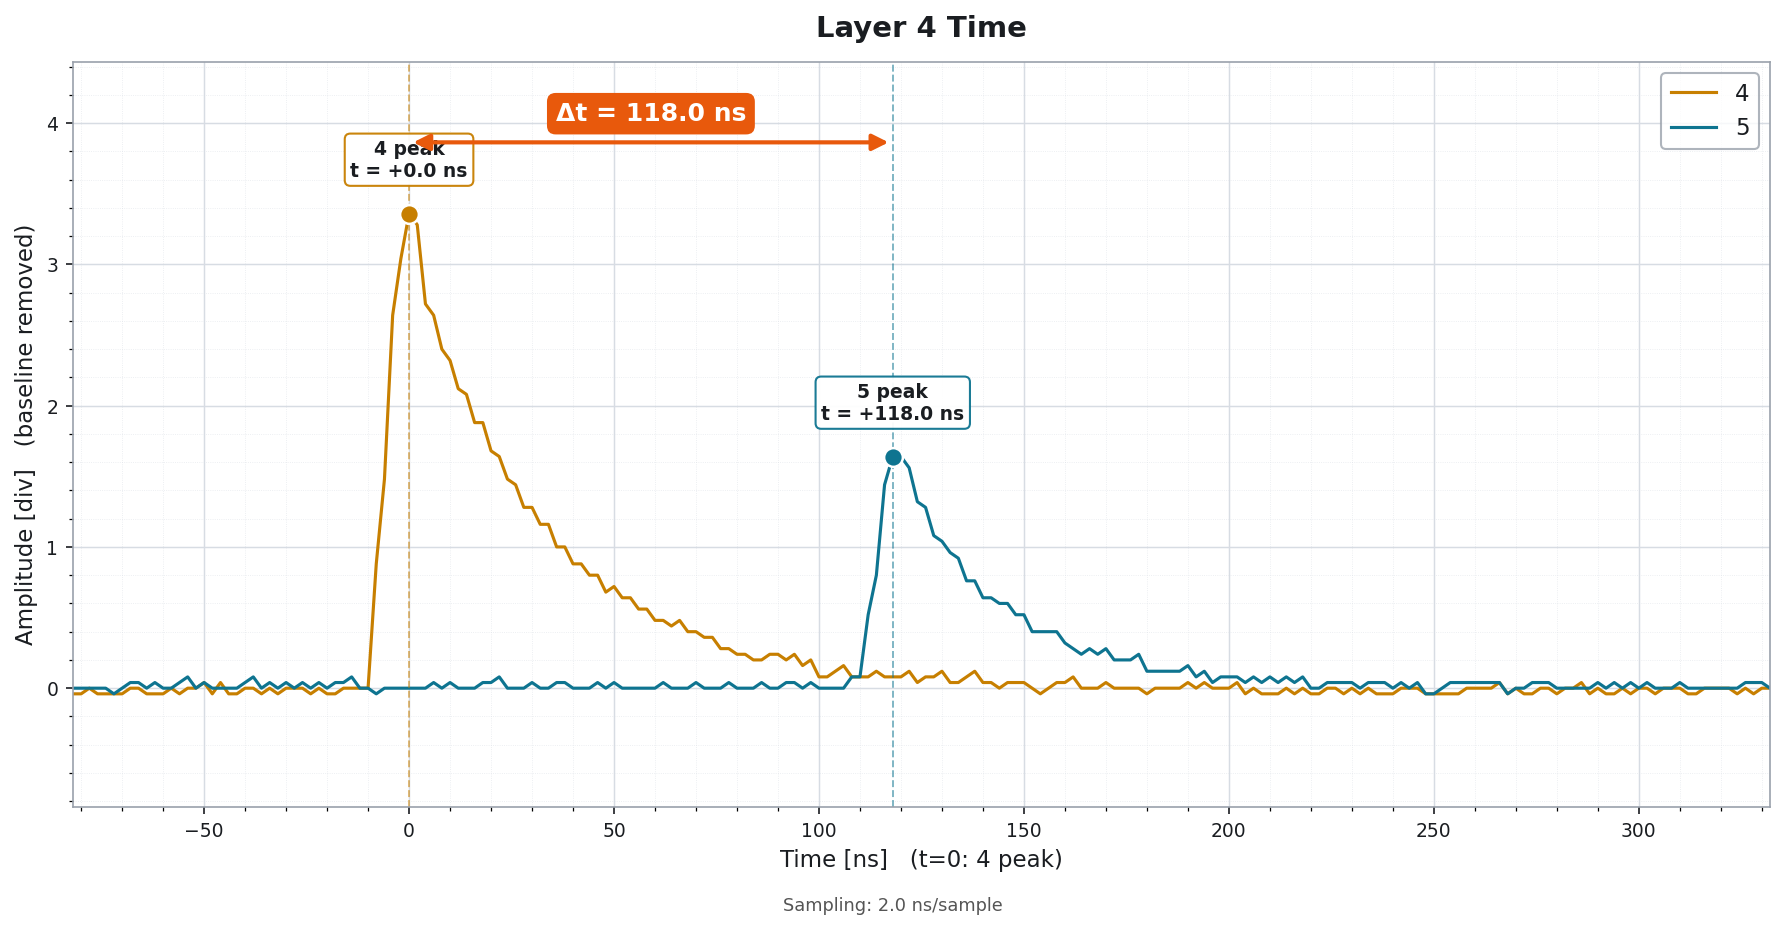
\includegraphics[width=0.49\linewidth]{figures/scope_layer4.png}
\caption{Oscilloscope captures of consecutive layer-done debug pulses; each
inter-pulse interval directly measures one layer's processing time. Top-left to
bottom-right: layer~1 (\SI{280}{\nano\second}), layer~2
(\SI{200}{\nano\second}), layer~3 (\SI{160}{\nano\second}), layer~4
(\SI{118}{\nano\second}).}
\label{fig:scope_layer}
\end{figure}

\begin{figure}[htbp]
\centering
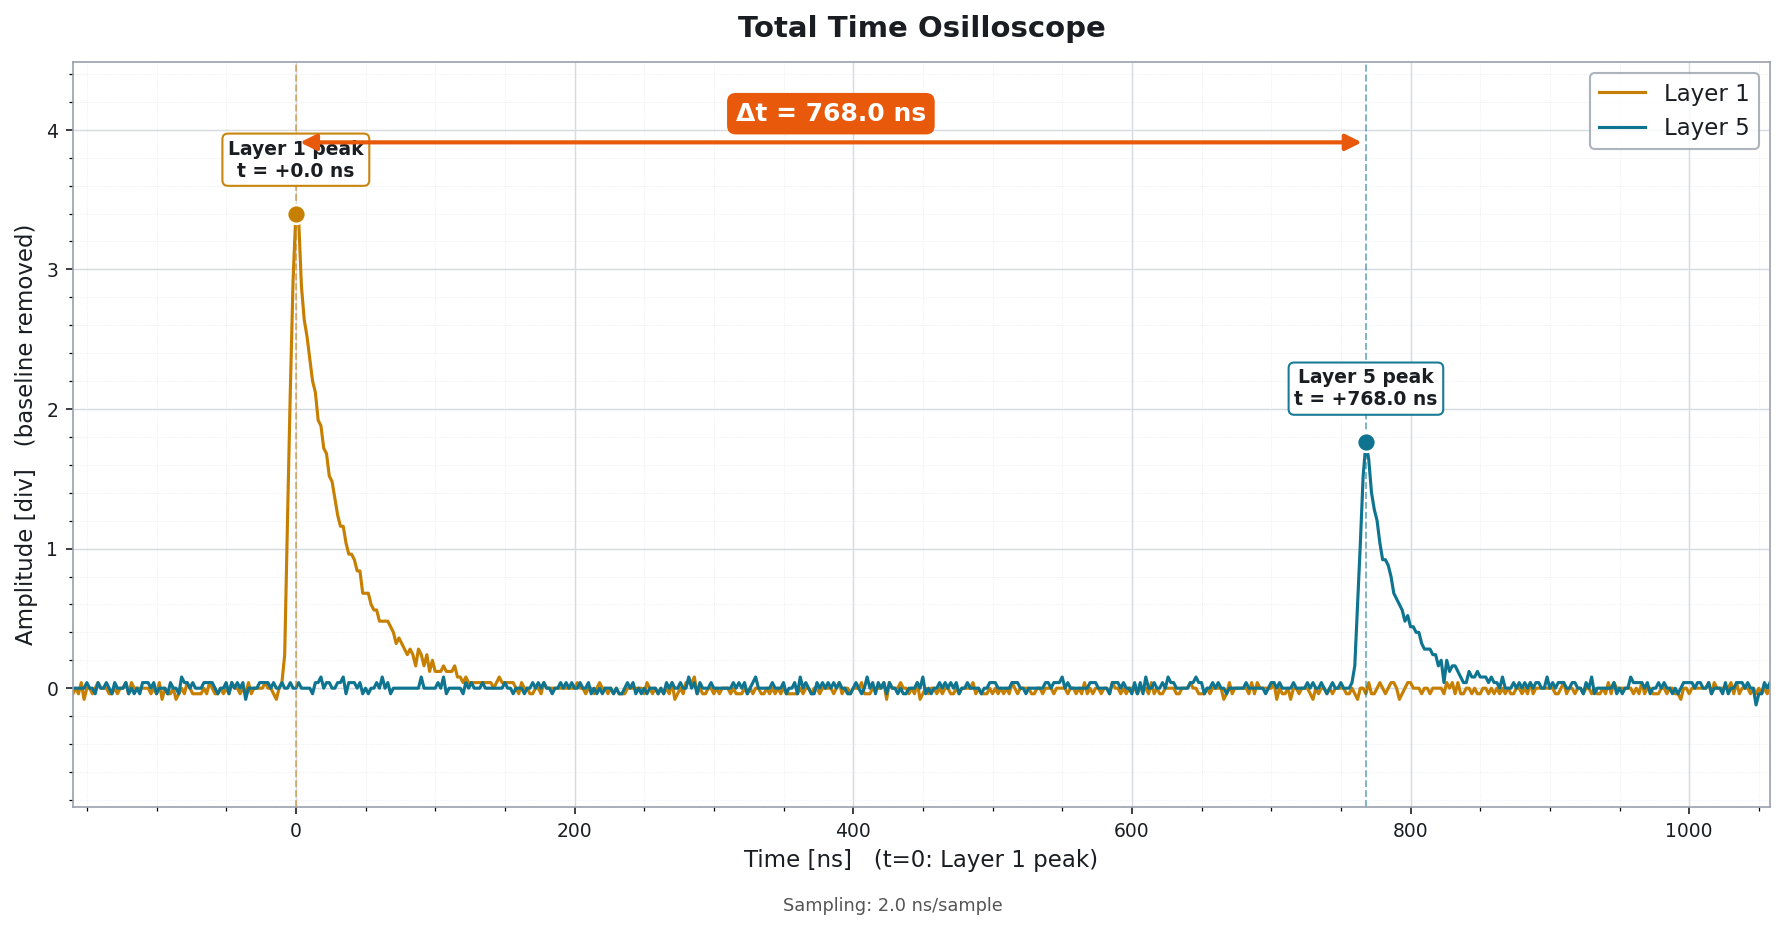
\includegraphics[width=\linewidth]{figures/scope_total.png}
\caption{Oscilloscope capture of the first and last debug pulses of an
inference, measuring the total hardware-core interval
($\Delta t = \SI{768}{\nano\second}$).}
\label{fig:scope_total}
\end{figure}

\begin{table*}[t]
\centering
\caption{Latency breakdown from Ethernet packet to trading decision, over a
1{,}004{,}229-packet run (all values in $\mu$s)}
\label{tab:latency_breakdown}
\begin{tabular}{p{4.6cm} p{1.5cm} p{2.4cm} p{4.4cm}}
\toprule
Stage & Mean & p50 / p99 & Measurement Method \\
\midrule
Ethernet packet reception (EMAC + lwIP) & 7.59 & 2.57 / 14.18 & PS timestamping (bimodal) \\
Packet parsing and buffer hand-off & 0.70 & 0.69 / 0.86 & PS timestamping \\
AXI-DMA transfer to PL & 3.70 & 3.70 / 3.78 & PS/PL counters \\
AXI-Stream receive + MLP core (PL) & 1.46 & 1.46 / 1.72 & \texttt{dbg} pins (core \SI{768}{\nano\second}) \\
Result readout & 0.96 & 0.96 / 0.97 & AXI-Lite \\
\midrule
Board subtotal (PS + PL) & 14.40 & 9.41 / 21.03 & On-board sum \\
Host end-to-end & 68.56 & 68.50 / 80.92 & Host round trip \\
\bottomrule
\end{tabular}
\end{table*}

\begin{table}[htbp]
\centering
\caption{Per-layer latency of the MLP core at \SI{125}{\mega\hertz}: analytic
prediction from \eqref{eq:cycles} against oscilloscope measurement on the
layer-done debug pins. Layers 1 to 4 are $40\!\rightarrow\!64$,
$64\!\rightarrow\!32$, $32\!\rightarrow\!16$ and $16\!\rightarrow\!3$
respectively.}
\label{tab:cycle_breakdown}
\small
\begin{tabular}{@{}lrrrrr@{}}
\toprule
 & & & \multicolumn{2}{c}{Predicted} & Meas. \\
\cmidrule(lr){4-5}
Layer & $n_\ell$ & $\lceil n_\ell/3\rceil$ & cyc & ns & ns \\
\midrule
1 & 64 & 22 & 36 & 288 & 280 \\
2 & 32 & 11 & 25 & 200 & 200 \\
3 & 16 &  6 & 20 & 160 & 160 \\
4 &  3 &  1 & 15 & 120 & 118 \\
\midrule
Total & \ & \ & 96 & 768 & 768 \\
\bottomrule
\end{tabular}
\end{table}

\subsection{Determinism of the Hardware Core}
\label{sec:determinism}
The claim that the core is deterministic has so far rested on oscilloscope
captures, which show one inference at a time and cannot exclude rare outliers.
To establish it over a population, a 16-bit cycle counter was added to the
engine. It is cleared when \texttt{start} is accepted, increments on every cycle
in which the controller is not idle, and is latched when the final layer asserts
\texttt{done}. The latched value is exposed at AXI-Lite offset \texttt{0x10} and
read back by the firmware after every inference, so each logged decision carries
the exact cycle count that produced it.

Over \num{100000} consecutive inferences driven at line rate the counter
returned 95 on every inference. Minimum, maximum and mean are all 95 and the
standard deviation is zero; the distribution has a single point of support. The
core therefore shows no jitter at all rather than a short tail: inference $k$ and
inference $k+1$ occupy the same number of cycles irrespective of the input
values, of the activation pattern, or of concurrent AXI-Lite and DMA traffic.
This is the property the application requires, since a trading system is exposed
to the worst case and not to the mean.

The counter reads 95 where \eqref{eq:cycles} predicts 96 because the two count
from different points. The counter increments only in non-idle cycles and is
latched on the same clock edge that returns the controller to the idle state, so
it excludes the cycle in which \texttt{start} is sampled; adding that cycle
gives 96, in agreement with both the analytic model and the
\SI{768}{\nano\second} interval measured on the debug pins
(Fig.~\ref{fig:scope_total}). The difference is a property of the instrument
rather than of the datapath, and the start-to-done convention is used
throughout.

\subsection{Comparison Against a Serial Baseline on the Same Device}
\label{sec:baseline}
The oscilloscope measurements establish that the hardware inference completes in
\SI{768}{\nano\second}, deterministically. Interpreting that number requires a
baseline, and the comparisons available in the literature are awkward: the
figures reported by other accelerators are measured between different points, on
different devices, for different networks. We therefore use a baseline that
removes all of these confounds: an earlier version of this same design, on
the same board, running the same network.

That earlier implementation is preserved in the version history of the artifact
and can therefore be characterised exactly rather than from recollection. It used
a sequential finite-state-machine controller driving a single
multiply-accumulate unit, with the same network dimensions hardwired into the
controller. Its cycle count follows directly from the state machine: each neuron
costs one cycle to load its bias, one cycle per input, and three further cycles
to apply the activation, write the result and advance, so a layer of $n_{\text{out}}$
neurons with $n_{\text{in}}$ inputs occupies $n_{\text{out}}(n_{\text{in}}+4)$
cycles. Summed over the four layers, with the layer transitions and the hardware
argmax included, the design required \num{5639} cycles per inference.

The comparison must be stated carefully, because the two designs did not run at
the same frequency: the sequential version was clocked at \SI{100}{\mega\hertz},
giving \SI{56.4}{\micro\second} per inference, whereas the present design closes
timing at \SI{125}{\mega\hertz}. Two speed-up figures follow, and they answer
different questions. Evaluated at a common \SI{125}{\mega\hertz} the sequential
design would require \SI{45.1}{\micro\second}, so the architectural change alone
accounts for a factor of $58.7$. As actually deployed, \SI{56.4}{\micro\second}
then against \SI{768}{\nano\second} now, the improvement is a factor of $73.4$,
of which the remainder is the higher clock. We quote the former where the
architecture is the subject.

Two mechanisms produce the gain, in unequal measure. Replacing the single MAC
unit with 192 parallel multipliers removes the serialisation of the arithmetic,
and replacing per-operand AXI-Lite writes with a DMA-fed stream removes a
processor transaction per input value. The second effect dominates: in the
sequential design the cost scaled with the \num{5168} multiply-accumulate
operations of the network rather than with its depth.

This is the most defensible speed-up figure in the paper, because it is derived
rather than measured under conditions we no longer control: the device, the
network and the measurement points are identical, the cycle count is recoverable
from the archived source, and the one confound that remains, the clock, is
separated out explicitly. The cross-platform comparisons of
Table~\ref{tab:related_work} deserve correspondingly more caution.

\subsection{Software Inference on the Same SoC}
\label{sec:arm_baseline}
The premise of the design is that moving inference off the processor and into
the fabric is worth the effort, and on this device that premise can be tested
directly, since the Zynq-7000 carries a \SI{667}{\mega\hertz} dual-core
Cortex-A9 alongside the fabric. The same network was therefore implemented in C
and run bare-metal on the PS using the same $Q8.8$ arithmetic as the hardware:
the same 40-bit accumulation, the same arithmetic right shift, the same
saturation, the same ReLU and the same argmax rule, with weights converted by
the same routine, so that the two paths compute identical values and differ only
in how the arithmetic is scheduled. Latency was measured with the Zynq Global
Timer over \num{1000} inferences with warm caches and with no network or DMA
activity inside the measured region.

The software path requires \SI{51.4}{\micro\second} per inference against
\SI{768}{\nano\second} in the fabric, a factor of $67$. Compilation settings
matter here and are worth stating explicitly: the identical source built without
optimization requires \SI{302}{\micro\second}, so a baseline left at the default
debug settings would have overstated the speed-up by almost a factor of six. The
figure reported here is compiled at \texttt{-O3}. It is scalar code; NEON
intrinsics were not hand-written, and even an optimiztic assumption of a further
factor of four from vectorisation would leave the fabric path ahead by roughly a
factor of 17.

One further comparison is worth drawing, because it sharpens what the
contribution actually is. The sequential hardware design of
Section~\ref{sec:baseline} required \SI{56.4}{\micro\second} as deployed, which
is slightly slower than optimized software on the same chip's processor. Moving
the computation into the fabric was therefore not by itself sufficient; a serial
datapath in logic bought nothing over a serial datapath in software. The gain
reported here comes from the parallel issue structure and from removing the
per-operand processor transactions, not from the change of substrate.

The comparison also has a dimension that latency alone does not express. The
software path occupies the processor for the whole \SI{51.4}{\micro\second}, and
during that interval it cannot service the network stack, whereas the hardware
path returns the processor to its polling loop as soon as the DMA descriptor is
posted. In a system whose residual latency is dominated by packet reception
(Table~\ref{tab:latency_breakdown}), that difference compounds.

\subsection{FPGA Resource Utilization}
Table~\ref{tab:resource_utilization} reports the post-implementation resource
usage on the XC7Z020, obtained from the post-implementation reports of the
verified design. The core is DSP-bound (\SI{87.3}{\percent}); logic usage
remains low (\SI{27.2}{\percent} of LUTs, \SI{10.7}{\percent} of flip-flops),
and \SI{70.4}{\percent} of the block-RAM tiles are occupied.

The block-RAM figure requires interpretation, because it does not indicate that
the memories are nearly full. As described in Section~\ref{sec:reconfig}, the
engine instantiates one memory per (neuron-slot, input) pair. Each of these 192
memories holds 128 words of 16 bits, i.e.\ \SI{2}{kbit} of an 18-kbit primitive.
The reported occupancy therefore counts \emph{tiles}, not stored data: roughly
\SI{88}{\percent} of the allocated block-RAM capacity is unused. Any increase in
the input width or in the number of parallel neurons multiplies the tile count
directly and exhausts the budget long before depth becomes a constraint.

\paragraph{Timing.}
All constraints are met at the \SI{125}{\mega\hertz} target
(\SI{8.000}{\nano\second} period), as summarized in Table~\ref{tab:timing}:
setup WNS \SI{0.038}{\nano\second}, hold WHS \SI{0.028}{\nano\second}, pulse
width WPWS \SI{3.020}{\nano\second}, with zero failing endpoints out of
31{,}828. The corresponding maximum frequency is \SI{125.6}{\mega\hertz}.

For a design whose multipliers are fully pipelined through the DSP input,
intermediate and output registers, this figure is lower than one would expect,
and the critical path explains why. The worst path does not lie in the
arithmetic at all: it runs from a payload register inside the AXI SmartConnect
to the enable input of one of the 192 weight memories, with a data-path delay of
\SI{7.298}{\nano\second} of which \SI{5.974}{\nano\second}
(\SI{81.9}{\percent}) is routing and only \SI{1.324}{\nano\second} is logic
across seven levels. The limiting factor is thus the physical distribution of
the AXI-Lite write path across a large number of small, spatially dispersed
memories, which is the same organizational choice identified above as the
scaling limit. Consolidating inputs into wider memory words would shorten this path and
raise the achievable frequency, in addition to relaxing the capacity bound; we
did not pursue it here because \SI{125}{\mega\hertz} is already supplied
directly by the PS clock generator and the core latency is not the dominant
term in the end-to-end path (Section~\ref{sec:eval}).

\paragraph{Power.}
Vivado's vectorless estimate for the implemented design is \SI{2.718}{\watt} of
total on-chip power (\SI{2.521}{\watt} dynamic, \SI{0.196}{\watt} static) at a
junction temperature of \SI{56.3}{\celsius}. We emphasise that this is a tool
estimate obtained by activity propagation rather than a measurement. The
breakdown in Table~\ref{tab:power} shows that the processing system accounts for
\SI{1.535}{\watt}, i.e.\ more than half of the total, while the entire
programmable-logic contribution (clocks, logic, signals, block RAM, DSP and
I/O) amounts to \SI{0.986}{\watt}. Comparisons against accelerator cards
should use the latter figure, since those designs do not include an application
processor in their reported power.

\begin{table}[htbp]
\centering
\caption{Post-implementation resource utilization on the Xilinx XC7Z020-1CLG484}
\label{tab:resource_utilization}
\begin{tabular}{lrrr}
\toprule
Resource & Used & Available & Utilization \\
\midrule
Slice LUTs        & 14{,}445 & 53{,}200  & 27.15\% \\
\quad as logic    & 14{,}361 & 53{,}200  & 26.99\% \\
\quad as memory   &       84 & 17{,}400  &  0.48\% \\
Slice registers   & 11{,}372 & 106{,}400 & 10.69\% \\
Block RAM tiles   &     98.5 & 140       & 70.36\% \\
DSP slices        &      192 & 220       & 87.27\% \\
Bonded IOB        &       14 & 200       &  7.00\% \\
BUFGCTRL          &        1 & 32        &  3.13\% \\
\bottomrule
\end{tabular}
\end{table}

\begin{table}[htbp]
\centering
\caption{Post-implementation timing closure at \SI{125}{\mega\hertz}
(\SI{8.000}{\nano\second} period, speed grade $-1$)}
\label{tab:timing}
\begin{tabular}{lrr}
\toprule
Check & Worst slack & Failing endpoints \\
\midrule
Setup (WNS)       & \SI{0.038}{\nano\second} & 0 / 31{,}828 \\
Hold (WHS)        & \SI{0.028}{\nano\second} & 0 / 31{,}828 \\
Pulse width (WPWS)& \SI{3.020}{\nano\second} & 0 / 12{,}091 \\
\bottomrule
\end{tabular}
\end{table}

\begin{table}[htbp]
\centering
\caption{On-chip power, Vivado vectorless estimate for the implemented design}
\label{tab:power}
\begin{tabular}{lr}
\toprule
Component & Power \\
\midrule
PS7 (processing system) & \SI{1.535}{\watt} \\
Signals                 & \SI{0.280}{\watt} \\
Block RAM               & \SI{0.249}{\watt} \\
DSP                     & \SI{0.236}{\watt} \\
Slice logic             & \SI{0.150}{\watt} \\
Clocks                  & \SI{0.066}{\watt} \\
I/O                     & \SI{0.005}{\watt} \\
\midrule
Dynamic total           & \SI{2.521}{\watt} \\
Device static           & \SI{0.196}{\watt} \\
\midrule
Total on-chip           & \SI{2.718}{\watt} \\
\quad of which PL only  & \SI{0.986}{\watt} \\
\bottomrule
\end{tabular}
\end{table}

\subsection{Deployment Cost}
The platform used here is a Digilent ZedBoard carrying an XC7Z020, a part in the
low hundreds of US dollars, against the several thousand typical of a
data-centre accelerator card. We deliberately avoid a tabulated cost comparison
against CPU, GPU and high-end FPGA alternatives, because we have not measured
this network on those platforms and a table populated with qualitative labels
would add nothing. What the measurements do support is narrower and can be
stated directly: a deterministic, sub-microsecond inference path for a network
of this size does not require a data-centre part. As a point of reference,
SparkNoC~\cite{sparknoc} reaches \SI{337.2}{GOP/s} at about \SI{7.6}{\watt} of
compute power on an Arria~10 GX1150 card, an order of magnitude more throughput
than the present design delivers, on hardware of a different class and for a
throughput-oriented workload rather than single-inference latency.

\subsection{Run-Time Reconfigurability and Scalability}
\label{sec:reconfig}
The framework property claimed in Section~\ref{sec:framework} is that a single
bitstream hosts different networks. This is not a matter of reloading weights
alone: the per-layer output widths are held in AXI-Lite configuration registers
that the issue FSM reads to derive its iteration counts, so the \emph{shape} of
the network is also a run-time parameter.

The verification campaign of Section~\ref{sec:verification} demonstrates this
directly. The four networks of Table~\ref{tab:verification} have different
hidden-layer widths, with the first hidden layer ranging from 10 to 64 neurons,
yet all four were loaded into the same programmed device over AXI-Lite and each
was verified bit-exactly. No re-synthesis, re-implementation or bitstream
reload took place between them; loading a network requires
$\sum_{\ell}\lceil n_\ell/3\rceil \times 3 \times 64$ weight writes plus the
corresponding biases, which for the reference topology is approximately
\num{7800} AXI-Lite transactions.

The limits of this reconfigurability should be stated precisely. The datapath is
elaborated for at most four layers, at most 64 neurons per layer and at most 64
inputs per layer; these bounds are compile-time constants of the SIMD array and
of the weight-memory instantiation. Any network within those bounds is hosted
without re-synthesis; a network exceeding them is not.

Scaling beyond these bounds is limited by memory organization rather than by
arithmetic. The design instantiates one memory per (neuron-slot, input) pair,
i.e.\ $\mathrm{PARALLEL\_NEURONS} \times \mathrm{MAX\_INPUTS} = 192$ weight
memories, each of which stores only 128 words and therefore occupies a small
fraction of the 18-kbit primitive it is mapped onto. The reported
\SI{70.4}{\percent} block-RAM occupancy thus reflects the \emph{number} of
memories rather than their depth: widening the input vector or increasing the
number of parallel neurons increases the block count proportionally and
exhausts the budget well before the depth of any individual memory becomes a
constraint. Packing several inputs per memory word is the natural way to relax
this limit and is left as future work.

%%%%%%%%%%%%%%%%%%%%%%%%%%%%%%%%%%%%%%%%%%%%%%%%%%%%%%%%%%%%%%%%%%%%%%%%%%%%%%%
\section{Discussion}
%%%%%%%%%%%%%%%%%%%%%%%%%%%%%%%%%%%%%%%%%%%%%%%%%%%%%%%%%%%%%%%%%%%%%%%%%%%%%%%
The results support three observations. First, embedding the network in the PL
makes the core latency a property of the pipeline rather than of the operating
system: the measured core latency is \SI{768}{\nano\second} and deterministic,
whereas the end-to-end host path around it varies from \SI{66}{} to
\SI{476}{\micro\second} in median across operating systems and shows heavy tails. Second, $Q8.8$ quantization is essentially
accuracy-neutral here (at most 0.22 percentage points across five models), so
the speed-up does not cost predictive quality. Third, the design fits a low-cost Zynq-7000 at \SI{2.72}{\watt} with
positive timing slack, so the approach does not depend on premium accelerator
hardware. The instrumented per-stage breakdown
(Table~\ref{tab:latency_breakdown}) further shows that only
\SI{14.4}{\micro\second} of the \SI{68.6}{\micro\second} end-to-end latency is
spent on the board, so the main remaining limitation is the host- and
network-side software path; moving the Ethernet stack into the PL is the clearest
next step.

%%%%%%%%%%%%%%%%%%%%%%%%%%%%%%%%%%%%%%%%%%%%%%%%%%%%%%%%%%%%%%%%%%%%%%%%%%%%%%%
\section{Conclusion}
%%%%%%%%%%%%%%%%%%%%%%%%%%%%%%%%%%%%%%%%%%%%%%%%%%%%%%%%%%%%%%%%%%%%%%%%%%%%%%%
We presented an Ethernet-fed MLP inference framework embedded in the
programmable logic of a low-cost Zynq-7000 SoC. Feature vectors are streamed to
the PL over AXI-DMA, and a 192-multiplier, 13-stage pipelined core performs the
$Q8.8$ inference in \SI{768}{\nano\second} with deterministic timing, using
\SI{27.2}{\percent} of the LUTs and \SI{87.3}{\percent} of the DSP slices of an
XC7Z020 at an estimated \SI{2.72}{\watt} of total on-chip power, of which
\SI{0.99}{\watt} is attributable to the programmable logic. The same network
executed bare-metal on the SoC's own Cortex-A9 requires
\SI{51.4}{\micro\second}, so moving the computation into the fabric is worth a
factor of $67$ against an independent baseline on identical arithmetic
(Section~\ref{sec:arm_baseline}). Decomposed against an earlier sequential
implementation of the same network on the same device, the architecture accounts
for a factor of $58.7$ at a common clock, and $73.4$ as the two were actually
deployed (Section~\ref{sec:baseline}).

The property that distinguishes the design from compiler-style FPGA inference
frameworks is that the network shape is a run-time rather than an
elaboration-time parameter: four networks with different hidden-layer widths
were deployed into one unchanged bitstream over AXI-Lite, with no synthesis step
between them.
Correctness of the deployed arithmetic is not assumed but established: the core
was verified bit-exactly against an independent reference model over 400{,}000
inferences, a process that first exposed and then eliminated three
pipeline-alignment defects that neither synthesis nor end-to-end testing had
revealed.

Two directions follow from the measured breakdown. First, only
\SI{14.4}{\micro\second} of the \SI{68.6}{\micro\second} end-to-end latency is
spent on the board, so integrating an Ethernet MAC directly in the programmable
logic, and thereby removing the host network stack from the path, is the change
with the largest remaining effect. Second, the present bounds on network shape
(at most four layers of at most 64 neurons and 64 inputs) follow from the
one-memory-per-input organization of the weight storage rather than from the
arithmetic; packing several inputs per memory word would relax them without
additional DSP cost.

%%%%%%%%%%%%%%%%%%%%%%%%%%%%%%%%%%%%%%%%%%%%%%%%%%%%%%%%%%%%%%%%%%%%%%%%%%%%%%%
% ELSEVIER ZORUNLU BEYANLARI
% Asagidakilerin hepsi JSA gonderiminde isteniyor. Metinleri kendi
% durumunuza gore duzenleyin; bos birakmayin.
%%%%%%%%%%%%%%%%%%%%%%%%%%%%%%%%%%%%%%%%%%%%%%%%%%%%%%%%%%%%%%%%%%%%%%%%%%%%%%%

\section*{CRediT authorship contribution statement}
\noindent
\textit{Ahmet Batuhan \"Ozkaner:} Conceptualization, Methodology, Software,
Validation, Formal analysis, Investigation, Data curation, Visualization,
Writing (original draft), Writing (review and editing).
\textit{Mustafa Alper Il{\i}k:} Software, Investigation,
Writing (review and editing).
\textit{Baykal Sar{\i}o\u{g}lu:} Supervision, Project administration.

\section*{Declaration of competing interest}
The authors declare that they have no known competing financial interests or
personal relationships that could have appeared to influence the work reported
in this paper.

\section*{Funding}
This research did not receive any specific grant from funding agencies in the
public, commercial, or not-for-profit sectors.

\section*{Data availability}
The artifact supporting this study is publicly available at
\url{https://github.com/ozkanerbatuhan/hft} (hardware) and
\url{https://github.com/ozkanerbatuhan/HFT_vitis} (firmware and host tooling).
It contains the RTL sources, the self-checking
testbench, the cycle-accurate reference model, the host and firmware tooling, the
stimulus generator, the post-implementation reports, and the measurement logs
behind the latency and verification results. Instructions for rebuilding the
bitstream and for reproducing each claim are given in the accompanying
documentation.

%%%%%%%%%%%%%%%%%%%%%%%%%%%%%%%%%%%%%%%%%%%%%%%%%%%%%%%%%%%%%%%%%%%%%%%%%%%%%%%
% REFERENCES
%%%%%%%%%%%%%%%%%%%%%%%%%%%%%%%%%%%%%%%%%%%%%%%%%%%%%%%%%%%%%%%%%%%%%%%%%%%%%%%
\bibliographystyle{elsarticle-num}
\bibliography{references}

\end{document}
